% Version 0; preprint format; Written by SH

\documentclass[preprint]{aastex}

% Packages
\usepackage{emulateapj5}
\usepackage{apjfonts}
\usepackage{amssymb, amsmath}
\usepackage{graphicx}
\usepackage{CJK}
\usepackage{natbib}
\usepackage{hyperref}
\usepackage[usenames]{color}

% Package Settings
\bibliographystyle{apj}
\hypersetup{colorlinks=true,
            citecolor=cyan,
            linkcolor=cyan,
            filecolor=magenta,      
            urlcolor=cyan}
\urlstyle{same}

% Figure extention
\DeclareGraphicsExtensions{.pdf,.png,.jpg}
\input psfig.tex

%%%%%%%%%%%%: User Defined Commands %%%%%%%%%%%%

% Song Huang's definition 
\def\arcsec{{\prime\prime}}
\def\arcmin{{\prime}}
\def\degree{{\circ}}
\def\h{\hskip -3 mm}
\def\aa{{A\&A}}
\def\aas{{ A\&AS}}
\def\aj{{AJ}}
\def\al{$\alpha$}
\def\bet{$\beta$}
\def\amin{$^\prime$}
\def\annrev{{ARA\&A}}
\def\apj{{ApJ}}
\def\apjs{{ApJS}}
\def\asec{$^{\prime\prime}$}
\def\deg{$^{\circ}$}
\def\ddeg{{\rlap.}$^{\circ}$}
\def\dsec{{\rlap.}$^{\prime\prime}$}
\def\cc{cm$^{-3}$}
\def\flamb{erg s$^{-1}$ cm$^{-2}$ \AA$^{-1}$}
\def\flux{erg s$^{-1}$ cm$^{-2}$}
\def\fnu{erg s$^{-1}$ cm$^{-2}$ Hz$^{-1}$}
\def\hst{{\textit{HST}}}
\def\kms{km s$^{-1}$}
\def\lamb{$\lambda$}
\def\lax{{$\mathrel{\hbox{\rlap{\hbox{\lower4pt\hbox{$\sim$}}}\hbox{$<$}}}$}}
\def\gax{{$\mathrel{\hbox{\rlap{\hbox{\lower4pt\hbox{$\sim$}}}\hbox{$>$}}}$}}
\def\simlt{\lower.5ex\hbox{$\; \buildrel < \over \sim \;$}}
\def\simgt{\lower.5ex\hbox{$\; \buildrel > \over \sim \;$}}
\def\micron{{$\mu$m}}
\def\mnras{{MNRAS}}
\def\nat{{Nature}}
\def\pasp{{PASP}}
\def\perang{\AA$^{-1}$}
\def\peryr{yr$^{-1}$}
\def\reference{\noindent\pp}
\def\refindent{\par\noindent\parskip=2pt\hangindent=3pc\hangafter=1 }
\def\sb{mag~arcsec$^{-2}$}
\def\lsun{$L_\odot$}
\def\msun{$M_\odot$}
\def\sigs{$\sigma_*$}
\newcommand{\lt}{<}
\newcommand{\gt}{>}

\def\etal{{\ et al.~}}
\def\galfit{{\tt GALFIT}}
\def\ser{{S\'{e}rsic\ }}
\def\redm{\texttt{redMaPPer}}
\def\redbcg{{$\Lambda \ge 30$}}
\def\nonbcg{{$\Lambda < 20$}}
\def\logms{{$\log (M_{\star}/M_{\odot})$}~}
\def\mstar{{$M_{\star}$}~}
\def\logmh{{$\log (M_{\mathrm{Halo}}/M_{\odot})$}~}
\def\m2l{{$M_{\star}/L_{\star}$}~}

% Commenting:
\newcommand{\todo}[1]{\textcolor{red}{\textbf{TODO:~#1}}}
\newcommand{\plan}[1]{\textcolor{cyan}{#1}}
\newcommand{\addref}{{\textcolor{red}{REF}}}
\newcommand{\note}[2]{\textcolor{blue}{\textbf{[Comment (#1): #2]}}}
\newcommand{\song}[1]{\textcolor{magenta}{\textbf{[Song: #1]}}}
\newcommand{\alexie}[1]{\textcolor{blue}{\textbf{[Alexie: #1]}}}
\newcommand{\kevin}[1]{\textcolor{green}{\textbf{[Kevin: #1]}}}

%%%%%%%%%%%%: Header and Version %%%%%%%%%%%%

\slugcomment{Draft version 0}
\email{song.huang@ipmu.jp}
\shorttitle{ENVIRONMENT DEPENDENCE OF MASS-SIZE RELATION}
\shortauthors{HUANG ET AL.}

\begin{document}

\begin{CJK*}{UTF8}{gbsn}

%%%%%%%%%%%%: Title and Affiliations %%%%%%%%%%%%

\title{The Environmental Dependence of Structures for Massive Galaxies
from the Hyper Suprime-Cam Survey}

\author{Song Huang (黄崧)\altaffilmark{1} 
        Alexie Leauthaud\altaffilmark{1}, 
        Kevin Bundy\altaffilmark{1},
        Michael Strauss\altaffilmark{2},
        Yen-Ting Lin\altaffilmark{3},
        Rachel Mandelbaum\altaffilmark{4}
        }
\date{}                                          

\altaffiltext{1}{Kavli Institute for the Physics and Mathematics of the 
    Universe, The University of Tokyo Institutes for Advanced Study, 
    the University of Tokyo (Kavli IPMU, WPI), Kashiwa 277--8583, Japan}
\altaffiltext{2}{Princeton University Observatory, 
    Peyton Hall, Princeton, NJ 08544, USA}
\altaffiltext{3}{Institute of Astronomy and Astrophysics, Academia Sinica, 
    P.O.~Box 23--141, Taipei 10617, Taiwan}
\altaffiltext{4}{Carnegie-Mellon University \todo{correct affiliation here}}

%%%%%%%%%%%%: Abstract and Keywords %%%%%%%%%%%%

\begin{abstract}
    \todo{Place holder; This is the abstract used for giving a talk.}\\
    Under the most popular formation scenario, the structures of massive central galaxies
    depend on environment at fixed stellar mass due to different assembly histories shaped
    by their host halos. Yet, clear evidence of such effect is still lacking. Using deep,
    multi-band images for a large sample of massive galaxies at 0.2 < z < 0.5 from the
    Hyper Suprime-Cam (HSC) survey, we discover subtle, but systematic structural
    difference for massive galaxies in low and high mass haloes. The differences are
    consistent with richer merger history in more massive halos. We show that the average
    profiles of mass, shape, and color, along with relations among masses within different
    radius (as proxy of mass assembled at different time) can help us gain more insights
    of their assembly history, and the weak lensing analysis enabled by HSC survey further
    helps us connect the differences we find to the average halo properties.
\end{abstract}
\keywords{galaxies: elliptical and lenticular, cD --- galaxies: formation --- 
          galaxies: photometry --- galaxies: structure --- galaxies: surveys}

\maketitle

%%%%%%%%%%%%: Main Text %%%%%%%%%%%%

%% ------------------------------------------------------------------------------------ %% 
\section{Introduction}

    \plan{Scientific Background}
    \begin{itemize}
        \item \plan{Massive galaxies are important cosmic probe and unique labs to study 
            galaxy evolution.} 
        \item \plan{Briefly explain why massive early-type galaxies are important through 
            the difficulties of stellar-halo mass relation and stellar mass function at the 
            high-mass end.}
        \item \plan{Brief summary of the current understanding of their cosmic assembly 
            history.}
        \item \plan{Explain why we should care about the environment, and why we expect to 
            see some environmental dependence in the structure and other properties of
            massive galaxies.}
        \item \plan{Brief review of the current observations.  It is still not clear 
            whether there is a clear environmental dependence.}
    \end{itemize}

    \plan{Observational difficulties (a.k.a Why we need HSC)}
    \begin{itemize}
        \item \plan{Explain why it is important to study the mass distribution of 
            massive galaxies out to large physical radius; and, given their unique light 
            profiles, why it is more difficult to study them compared to late-type 
            galaxies.}
        \item \plan{Very brief summary of past observational efforts, and why they are not 
            good enough (Not enough number of really massive galaxy; Shallow images; 
            Background subtraction issue; and stacking analysis can be dangerous as while)}
    \end{itemize}
    
    \plan{Basic idea of this work}
    \begin{itemize}
        \item \plan{Here we take advantages of the ambitious Hyper-Suprime camera 
            survey\ldots}
    \end{itemize}

    The paper is organized as follows. Section~2 gives a brief overview of the HSC
    observation and data reduction.  We will also summarize the process of sample
    selection.  In Section~3, we will describe the method for deriving the stellar mass 
    surface density profile.  The main results are summarized in Section~4.  Section~5 
    provides discussions of the assumptions used in this work, the potentially interesting
    physical implications, and several future improvements, ending with a summary in
    Section~6.

    All the magnitudes used here are in AB system (\citealt{Oke1983}), and are corrected 
    for Galactic extinction using calibrations from \citet{Schlafly11}.
    Within this work, we assume $H_0$ = 70~km~s$^{-1}$ Mpc$^{-1}$, ${\Omega}_m=0.3$, 
    and ${\Omega}_{\Lambda}=0.7$. 
    
%% ------------------------------------------------------------------------------------ %% 

\section{Observations and Sample Selection}

\subsection{The Hyper Suprime-Cam Survey}

    The Subaru Strategic Program (SSP, \addref) makes use of the new prime-focus camera,
    the Hyper Suprime-Cam (HSC;~\citealt{Miyazaki2012}), on the 8.2-m Subaru
    telescope at Mauna Kea.  
    Taking advantage of the large field of view (FoV;~1.5 deg in diameter) of HSC, this
    ambitious multi-layer photometric survey will cover $\sim 1400$ deg$^2$ of sky in 5
    broad bands (\textit{g r i z Y}) to the depth of $r \sim 26$ mag in the \texttt{WIDE}
    part in the next few years.  
    This work is based on the internal data release \texttt{S15B}, which covers $\sim 100$
    square of degree of sky in all 5-band to the required depth of \texttt{WIDE} survey.  
    The regions covered by this release are overlapped with several previous spectroscopic
    survey (e.g. SDSS/BOSS: \citealt{Eisenstein2011}, \citealt{Alam2015}; 
    GAMA: \citealt{Driver2011}, \citealt{Liske2015}).

    The data are processed with \texttt{hscPipe 4.0.1}, a derivative of the Large Synoptic
    Survey Telescope (LSST) pipeline (e.g. \citealt{Ivezic2008}; \citealt{Axelrod2010}),
    modified for use with Suprime-Cam and Hyper Suprime-Cam.  
    \texttt{hscPipe} first bias subtract, flat field, model background, and perform object
    detection and measurement on the single exposure data. 
    Then, different exposures are warped onto a common World Coordinate System (WCS) and
    combined into final images with improved signal-to-noise ratio (SNR) after astrometric
    and photometric calibration.  
    The pixel scale of the combined images is $0.168^{\arcsec}$.  
    The photometric calibration is based on data obtained from the Panoramic Survey 
    Telescope and Rapid Response System (Pan-STARRS) 1 imaging survey 
    (\citealt{Schlafly2012}, \citealt{Tonry2012}, \citealt{Magnier2013}). 
    To achieve consistent deblending and photometry across all bands, the \texttt{hscPipe}
    will perform multi-band post-processing on the combined images.  
    The footprints and peaks of detected sources on each band will be merged into a single
    catalog.    
    This consistent set of peaks and footprints is used as starting point for deblend and
    measure objects on the combined images of each band.  
    These measurements are then merged into a reference catalog.  After fixing the
    centroids, shape, and other non-amplitude parameters of every object in this catalog,
    \texttt{hscPipe} will derive forced photometry measurements at each band. 
    Details of \texttt{hscPipe} and the multi-band processing method will be presented in
    \addref~(Bosch\etal~in prep.).     
          
    In Figure 1, we compare the false color ({\tt gri}) images of three nearby massive
    ETGs from both SDSS and HSC surveys.  
    The images are generated using similar scaling and color schemes, and clearly
    demonstrate HSC's capability to reach to low surface brightness domain.  
    In $i$-band (ignoring the slight difference in filter response curve), the HSC
    \texttt{WIDE} image is $2.5$-$3.0$ magnitude deeper than SDSS on average.  
    This gives us huge advantage in exploring the outskirt of massive ETGs given their
    extended, shallow outer surface brightness profiles. 
    
    Motivated by the requirement of weak lensing analysis, the $i$-band data typically has
    the best seeing in all five bands (the median seeing is around 
    FWHM$\sim 0.8^{\arcsec}$).
    Therefore, we will mostly use the $i$-band images to study the structure of galaxies. 
    
\subsection{Massive Central Galaxies in Different Environments}

    The main scientific goal of this work is to investigate mass assembly history of
    massive, central ETGs, and its dependence on environments (or host dark halo mass)
    through their the spatial distribution of stellar mass.  
    
    To achieve this goal, we will select \logms$ > 11.5$ massive central galaxies within
    host halo mass larger and smaller than \logmh$= 14.0$ at $0.3 < z < 0.5$.  
    As both $M_{\star}$-$M_{\mathrm{Halo}}$ relation and stellar mass function are still
    quite uncertain at \logms$ > 11.5$, it is of great interest to investigate the
    structure of galaxies in this region carefully.
    And, this stellar mass cut can greatly reduce the contamination of satellites (e.g.
    \citealt{vanUitert2016}).  
    Meanwhile, under the adopted cosmology, $1.0^{\arcsec}$ equals 4.4 and 6.1 kpc at 
    redshit 0.3 and 0.5.  
    Therefore, this redshift range enables us to reliable measure the total stellar mass 
    within the inner 5 to 10 kpc (where the ``in-situ'' component should still dominates) 
    of massive galaxies at the high redshift end assuming the typical seeing of HSC data. 
    At the same time, the depth of the data still allows to study the very outskirt ($\sim
    100$ kpc) of these galaxies at $z\sim 0.5$.  
    Also, such limits on mass and redshift ensure us a sizeable sample while let us 
    safely ignore significant mass growth and structural evolution 
    (no star formation, lower merger rate \etal~e.g.
    \citealt{Bellstedt2016}, \citealt{Inagaki2015}; but also see \citealt{Bai2014}; 
    more discussion about this in Section~5). 
        
    Based on recent constraints of $M_{\star}$-$M_{\mathrm{Halo}}$ relation 
    (e.g. \citealt{Leauthaud2012}, \citealt{Behroozi2013}, \citealt{Kravtsov2014}), 
    above \logms$ = 11.5$, there is a large scatter of halo mass at fixed stellar mass.  
    At \logmh$<14.0$, these massive galaxies are mostly the centrals of small groups;
    while at \logmh$>14.0$, they start to become the centrals of very massive groups and
    galaxy clusters.   
    Limited by the sample size and the capability of measuring halo mass for individual
    central galaxy, we will simply separate the sample into two broad halo mass bins with
    the help of the \redm{} cluster catalog\footnote{See:
    http://risa.stanford.edu/redmapper/} (\texttt{v5.10}, e.g. \citealt{Rykoff2014};
    \citealt{Rozo2015b}).
    These clusters are selected from the SDSS DR8 photometric data using overdensity of
    red-sequence galaxies. 
    For each cluster, the catalog provides robust estimations of photometric redshift
    $z_{\Lambda}$ and richness $\Lambda$, along with the best candidate of the central
    galaxy (the one with the highest central probability \texttt{P\_CEN}).
    Information about the identified member candidates is also provided separately. 
    Please see \citet{Rozo2014}, \citet{Rozo2015a}, \citet{Rozo2015b} for more details 
    about the performance of the \redm~cluster catalog.      
    Several works (e.g. \citealt{Saro2015}; \citealt{Farahi2016}; \citealt{Simet2016})
    have tried to calibrate the $M_{200, c}-\Lambda$ relation using different methods.
    Despite the slightly different calibrations derived, it is safe to assume that most
    clusters identified by \redm~($\Lambda > 20$) have $\log (M_{200,c}/M_{\odot}) \geq
    14.0$.  
    Considering the typical uncertainty of richness, and the fact that \redm~catalog
    starts to become incomplete toward low richness ($\Lambda < 40$) end at $z > 0.33$, we
    will focus on the $\Lambda > 30$ clusters in this work.  
    Based on the calibrations from \citet{Farahi2016} or \citet{Simet2016}, 
    such richness cut gives us haloes with 
    $M_{200c} \geq 1.56\pm0.35 \times 10^{14} M_{\odot}$ or 
    $M_{200c} \geq 1.60\pm0.11 \times 10^{14} M_{\odot}$.  
    Therefore, \redm~can provide us a sample of massive central galaxies in \logmh$\geq
    14.0$ haloes.  
    And, we assume that, in the same footprints and redshift range, the \logms$\geq 11.5$
    galaxies outside \redm~clusters are most likely to be the central of \logmh$< 14.0$
    haloes. 
    
    According to Leauthaud\etal~(2016), all $0.3 < z < 0.5$ and \logms$\geq 11.5$ galaxies
    should have $i_{\mathrm{SDSS, cModel}} \leq 21.0$ mag.  Ignoring the tiny difference
    in response curves between SDSS and HSC $i$-band filters, we started by selecting all
    galaxies with $i_{\mathrm{HSC, cModel}} \leq 21.5$ in the regions that are covered in
    all five filters, and have already reached the expected depth of \texttt{WIDE} survey.  
    %% The SQL search is saved as "sample.sql" 
    %% The master catalog used here is "dr1_wide_galaxy_icmodel_21.5.fits"
    %%   The original catalogs contain 2275477 objects
    The details of the HSC \texttt{cModel} photometry, and its performence will be
    described in \addref~Bosch\etal~in.\ prep. 
    It is quite similar to the SDSS \texttt{cModel} in principle as it also fits the total
    flux of an object using a combination of de~Vaucouleur and exponential components
    after the PSF convolution is considered.  
    For this work, we select objects that are classified as extended, have well defined 
    centroids, do not fail during the deblending process, and have \texttt{cModel} 
    magnitudes in all five bands. 
    \song{Should we discuss the impact of failed cModel photometry?} 
    A series of quality control cuts are applied to remove objects that are affected by 
    saturation, cosmic ray, other optical artifacts; and the ones that are too close to 
    the edge of the field in all five bands 
    (each criterion affects less than 8\% of the entire sample).
    After these cuts, a total number of 1760845 galaxies left in the sample.
    This sample will be referred as \texttt{hscPho}. 
    %% Saved as "dr1_wide_galaxy_hscPho.fits"
    
    We match this sample with the central galaxies of \redm~catalogs using a 
    $1.0^{\arcsec}$ radius, and it results in 704 galaxies.  
    %% Saved as "dr1_redbcg_hsc_sdss_gama_1arcsec.fits"
    A small fraction of \redm~centrals in the our footprints do not have matched object in
    our sample due to severe contamination from optical artifacts or bleeding trails from
    saturated objects.  
    And slight change of the matching radius has no impact of this sample.  
    For galaxy in this sample, the photometric redshift of the cluster is available for
    each of them; and for 72\% of them, the spectroscopic redshift from SDSS DR8 is also
    provided by \redm~catalog when available. 
    This sample of will be referred as \texttt{redBCG} in the rest of the paper.
    
    For the vast majority of galaxies that are not the centrals of very massive haloes, we
    need other sources for their redshift estimations. 
    Although there has been many efforts for deriving photometric redshift (photo-$z$)
    using HSC five-band photometry, it is still a working progress now, and its
    performance at $z \leq 0.5$ is expected to be less satisfying due to the lack of
    information at the shorter wavelength side of the 4000$\AA$ break.  
    Therefore, we will only rely on external spectroscopic redshifts (spec-$z$) for this
    work.  
    The HSC database compiles a catalog of external spec-$z$ for this data release by
    matching the detected objects with public data of several spectroscopic surveys (e.g.
    SDSS/BOSS; GAMA). 
    Duplicated matches from different sources are merged through internal matching using
    $0.5^{\arcsec}$ radius. 
    For each object, the quality information of the spec-$z$ from different catalogs are 
    homogenized into a single flag that indicates whether the redshift is secure, and 
    only secure spec-$z$ are used in this work. 
    %% This is catalog: "dr1_specz_use.fits"
    
    We match the \texttt{hscPho} sample with this external spec-$z$ catalog using a 
    $1.0^{\arcsec}$ radius, and it leads to 116813 matched objects.  
    %% Saved as "dr1_wide_galaxy_icmodel_21.5.fits"
    Among these matches, there are 42696 objects at $0.3 \leq z \leq 0.5$. 
    Most of these redshifts come from either SDSS or GAMA survey.
    To further exclude contamination from satellite galaxies, we aggressively remove 
    all galaxies that could be associated with the \redm~clusters from this catalog.  
    First, the catalog of \texttt{redBCG} central galaxies is merged with the catalog  
    of their member galaxies. 
    Then, through cross matching using $1.0^{\arcsec}$ radius, all \texttt{hscPho} 
    galaxies that are within 2.5 Mpc of projected distance to any of cluster member 
    are removed from the catalog.  
    After this step, 29973 galaxies are left in the sample. 
    We will refer this sample as \texttt{nonBCG} later.
    %% Saved as "dr1_nonbcg_use_sed5b.fits"

    The \texttt{redBCG} sample is also matched with external spec-$z$ catalog in the same
    way, and we update the redshift of the central galaxies with external spec-$z$ when 
    it is available.  
    For the unmatched ones, 3 of them have spec-$z$ of BCG provided by the \redm~catalog 
    (most likely due to different criteria during the selection of spec-$z$ sample).
    For the rest, we use the photo-$z$ of the cluster from the \redm~catalog instead.
    At $0.3 \leq z \leq 0.5$, there are 375 central galaxies left in the \texttt{redBCG} 
    sample. 
    Among them, 67 (17.9\%) do not have spec-$z$.
    Using the central galaxies that have both spec- and photo-$z$, we estimate the median 
    absolute redshift difference $|z_{\mathrm{Photo}} - z_{\mathrm{Spec}}|$ is 
    $\sim 0.01$ (only 12 have absolute difference larger than 0.05; and the largest 
    difference is $\sim 0.12$).  
    Therefore, we expect the mixture of \redm photo-$z$ and spec-$z$ results in no bias 
    for the \texttt{redBCG} sample given the goal of this work.  
    
    At the same time, the spec-$z$ for both \texttt{redBCG} and \texttt{nonBCG} samples
    both come from a heterogeneous catalog, which mainly consists of spec-$z$ from 
    SDSS/BOSS and GAMA survey. 
    All the current HSC \texttt{WIDE} footprints overlap with the SDSS/BOSS survey, 
    which is the most important spec-$z$ sources for this work.  
    As the main scientific goal of BOSS survey is to use the spatial distribution of
    Luminous Red Galaxies (LRG) to map the large scale structure, it selects a large
    sample of massive ETGs in our redshift range.  
    However, due to the complex selection criteria for different subsamples (e.g.\ 
    the LOWZ and CMASS), its \mstar completeness is not easy to estimate.  
    Recently, through comparing with the Stripe 82 Massive Galaxy Catalog
    (\texttt{S82-MGC}; \citealt{Bundy2015}), \citet{Leauthaud2016} suggests that the 
    BOSS spec-$z$ is about 80\% complete at \logms$\geq 11.6$ at $0.3 < z < 0.5$. 
    The current \texttt{WIDE} data also greatly overlap with the GAMA survey in the
    G09, G12, and G15 fields. 
    Thanks to the optimized spatial completeness and deeper limit magnitude in 
    $r$-band ($\sim 19.8$ mag) of the GAMA survey, it provides 14\% of additional
    spec-$z$ for our samples.  
    However, due to the selection on fixed magnitude, its \mstar completeness 
    strongly depends on redshift and optical color.  
    According to \citet{Taylor2011} (e.g.\ their Figure~6), the 80\% completeness 
    increases from $10^{10.8}$\msun at $z\sim 0.3$ to $10^{12.0}$\msun at $z\sim 0.5$.
    Although there must be systematic differences between the above two works, 
    we can expect a reasonable overall \mstar completeness ($\sim 80$\%) for our 
    samples at \logms$\geq 11.6$.  
    Later, we will further investigate the \mstar completeness and the impact of deeper
    photometry on total stellar mass estimate. 
    Considering the subtle differences in sources of redshift and \mstar completeness   
    between the \texttt{redBCG} and \texttt{nonBCG} samples, we will carefully 
    match them in the \mstar-$z$ space before any comparison is conducted.    
    %% Saved as "dr1_redbcg_use_sed5b.fits"

\subsection{Stellar Masses from SED Fitting}

    To further select galaxies that are truly very massive central galaxies, we use 
    the broadband Spectral Energy Distributions (SEDs) fitting (see 
    \citealt{Walcher2011} for a recent review) code 
    \texttt{iSEDFit}\footnote{http://www.sos.siena.edu/~jmoustakas/isedfit/} 
    (\citealt{Moustakas2013}) to provide estimations of average stellar 
    mass-to-light ratio (\m2l) and $k$-corrected photometry of our 
    sample. 
    \texttt{iSEDFit} takes a simplified Bayesian approach. 
    In general, it first generates a large grid of SEDs from synthetic stellar 
    population models by drawing randomly from the prior distributions of relevant 
    parameters (e.g.\ age, metallicity, dust extinction, and star formation history).
    Based on these models, it uses the observed photometry and redshift to 
    compute the statistical likelihood, and generate the posterior probability 
    distribution (PDF) functions of each parameter.  
    To get the best estimate of certain parameter, \texttt{iSEDFit} ``integrates'' 
    the full PDF over all the other ``nuisance'' parameters.
    Then, the median value of the resulting marginalized PDF is used as the best
    value, while the 1-$\sigma$ uncertainty is derived from the cumulative PDF.
    Please refer to \citet{Moustakas2013} for technical details and performance of     
    \texttt{iSEDFit}. 
    In this work, we derive average \m2l using the Flexible Stellar Population 
    Synthesis\footnote{http://scholar.harvard.edu/cconroy/sps-models}
    (FSPS; \texttt{v2.4}; \citealt{FSPS}, \citealt{Conroy2010}) model based on 
    the MILES\footnote{http://www.iac.es/proyecto/miles/pages/stellar-libraries/miles-library.php}
    (\citealt{MILES1}, \citealt{MILES2}) stellar library and \citet{Chabrier2003} 
    IMF between 0.1 to 100 \msun. 
    We use the delayed-$\tau$ model with stochastic star burst as the form of 
    star formation history (SFH).  
    We adopt flat distribution between 0.5 to 14.0 Gyrs as prior for the look-back 
    time when the star formation turned on. 
    The exponential delayed time-scale ($\tau$) is allowed to change between 
    0.1 to 3.0 with equal probability.  
    The chance of random star burst is set at 0.2 for every 2 Gyrs. 
    The duration of the star burst is draw from a logarithmic distribution 
    between 0.03 to 0.3 Gyr; and the mass fraction formed in the burst is from 
    a logarithmic distribution between 0.01 and 1.0.  
    Such form of SFH is generally considered to be appropriate for massive 
    quiescent galaxies at low redshift (e.g. \citealt{Kauffmann2003}). 
    For stellar metallicity, we assume flat distribution between 0.004 to 
    0.03 (which is the highest metallicity allowed by FSPS models).  
    And, the \citet{Calzetti2000} extinction law is adopted with a order two 
    Gamma distribution of $A_{V}$ between 0 to 2 magnitude.  
    To achieve reasonably good sampling across these parameters, we generate 
    250000 models using \texttt{iSEDFit}. 
    
    In principle, these choices of priors could leave systematic effects in 
    the estimate of stellar mass (e.g.\ \citealt{Bernardi2016b}). 
    For low-$z$ massive ETGs like the ones in our sample, the details form of 
    SFH, importance of random star burst, and the dust extinction should not be 
    major concern.  
    However, the choices of stellar population models and IMF can still 
    change the results systematically. 
    More discussions on this can be found in Appendix~A. 
    In short: 
    \begin{enumerate}
        \item Both \texttt{FSPS+MILES} and \texttt{BC03} (\citealt{BC03} models 
            still have difficulties recovering the optical color involving filters 
            at the red end (e.g~$i-$Y), which could relate to the challenge for 
            modern stellar population models to reproduce the optical color-color 
            relation of red-sequence galaxies (e.g. \citealt{MIUSCAT2}), or the 
            shallower photometry of HSC-Y band data. 
        \item The \texttt{BC03} provides slightly better overall ${\chi}^2$ and 
            systematically smaller \mstar than the \texttt{FSPS+MILES} models.  
            However, it is possible that the \texttt{BC03} model tends to 
            underestimate the \m2l for a fraction of them as the estimate 
            stellar age is unrealistically young for red, massive galaxies.  
            Therefore, we still use the \texttt{FSPS+MILES} model as the fiducial 
            one.  But, switching to the \texttt{BC03} model will not change any 
            key result in this work. 
        \item The usage of \citet{Salpeter1955} IMF results in systematically 
            higher \mstar (on average $+0.25$ dex of \logms).  
            Although there are multiple lines of evidence that favor Salpeter 
            or even more ``bottom-heavy'' IMF in the most massive ETGs 
            (e.g. \citealt{Conroy2012}; \citealt{Cappellari2012}), we still 
            present the main results using Chabrier IMF to accommodate galaxies 
            with lower \mstar in the sample, and to be as consistent as possible 
            with a few other works.  
            Also, the choice of IMF does not impact our results qualitatively.     
    \end{enumerate}
    
    Besides the priors for stellar population properties, different treatments of 
    the light profile and accuracy of sky background subtraction are also important
    for the estimate of \mstar as they strongly impact the estimate of total luminosity
    (e.g.\ \citealt{Bernardi2013} and \citealt{DSouza2015}).  
    At the depth of SDSS, the default \texttt{cModel} photometry is already shown to 
    be not very accurate at high-\mstar end (e.g. \citealt{Meert2015}; 
    \citealt{Bernardi2016a}) as it does not capture the extended envelope of these 
    galaxies. 
    As for HSC, it is much more challenging for \texttt{cModel} to recover the total 
    luminosity of massive ETGs since the stellar envelope becomes even more 
    extended for neither de~Vaucouleur or exponential model to reproduce.  
    However, the HSC \texttt{cModel} under the force-photometry mode can measure 
    \textbf{average} color of the galaxy with great accuracy (e.g. Huang\etal~in prep.~), 
    and provide us a reliable SED to estimate the \textbf{average} \m2l. 
    Considering this, we separate the process of estimating the total \mstar of 
    massive ETGs in our sample into two steps: 
    
    \begin{enumerate}
        \item Firstly, using the redshift and \texttt{cModel} magnitude in five bands, 
            we derive an initial estimate of the \mstar of the galaxy.  
            More importantly, we derive the \textbf{average} \m2l in $i$-band of the 
            galaxy, and use the best-fit SED to provide $k$-correction to the photometry.  
        \item In the next section, we will derive better estimate of total \mstar using 
            the more accurate total luminosity in $i$-band from integration of carefully 
            measured 1-D surface brightness profile, and the average \m2l from the SED
            fitting.  
    \end{enumerate}
    
    We choose $i$-band because it typically has the best seeing and image quality among 
    all five bands, and within our redshift range, the $i$-band data can still be seen 
    as reasonable tracer of underlying stellar mass distributions in rest-frame 
    (at least for massive ETGs).
    In practice, the accuracy of this approach depends on the reliability of the average
    \m2l, and whether the \m2l of the extended envelope missed by \texttt{cModel} is 
    similar to the average \m2l from the inner part.  
    It is well known that massive ETGs have negative optical color gradient which 
    indicates a gradient of \m2l (e.g.~\citealt{LaBarbera2012}; \citealt{DSouza2015}). 
    Although the color gradient at the very outskirt are still not well quantified, 
    it is believed to be smooth and shallow, which is favoured by our method.  
    Also, since we focus on the comparison between the \texttt{redBCG} and 
    \texttt{nonBCG}, our results should remain intact as long as there is no significant
    differences of color gradient between these two samples. 
    We will discuss more later but the initial result suggests that this is indeed the 
    case.  
    In principle, this is similar to the method adopted by the GAMA survey 
    (\citealt{Taylor2011}), where the average \m2l comes from SED fitting of 
    PSF-matched aperture photometry from multi-band photometry while the better total
    luminosity relies on multi-band \ser model fitting (\citealt{Kelvin2012}).  

    \song{Not sure if we want to show this here, but just leave it here for now.}
    The basic results from \texttt{iSEDFit} are summarized in Figure~2, where we compare
    the relations between initial estimates of \mstar and (both luminosity and 
    star formation weighted) stellar age, metallicity, and dust extinction. 
    As expected, most galaxies in our samples are 
    $\log(M_{\star,\ \mathrm{ini}}/M_{\odot}) \geq 11.2$ massive galaxies that have 
    old age, high metallicity ($1.5 \times Z_{\odot}$ is the highest metallicity allowed), 
    and low dust extinction.  
    Given that we only have photometry from five optical bands, degeneracies among 
    age, metallicity, and dust extinction are naturally expected.  
    We will not use them for any scientific reason in this work, but to show that they
    behave reasonably.   
    
    Currently, the \texttt{cModel} photometry heavily underestimates the 
    flux errors of bright objects like the low-$z$ massive galaxies in our samples 
    since it only considers the statistical error of the data, not the systematic 
    uncertainties within the model-fitting process.  
    Therefore such flux errors are not useful here as they leads to strongly biased
    PDF for \mstar.  
    Photometric tests using simulated galaxies suggest that, even at the very bright 
    end, the average accuracy of \texttt{cModel} photometry is not better than 1\%.  
    Based on that, we supply \texttt{iSEDFit} with simplified flux errors assuming 
    $S/N = 100$ for $riz$ bands, and $S/N = 80$ for $gY$ bands (that typically 
    have shallower images).  
    Given such assumption, the typical uncertainty of \logms for both samples is 
    around 0.08 to 0.10 dex at the high-\mstar end. 
    
    From the \texttt{iSEDFit} results, we also derive the $k$-corrected luminosity and 
    colors.  
    \song{Will modify the Fig3c to only show the g-r and g-z color, and remove the 
    dashed vertical lines, replace them with single vertical line indicating logm=11.6; 
    r-z and i-y are just to show the problem of SED fitting at the red end}
    In Figure~3, we show the $M_{\star,\ \mathrm{ini}}$-color relations for 
    $k$-corrected $g-r$ and $g-z$ colors, and compare their distributions for 
    \texttt{redBCG} and \texttt{nonBCG} samples at 
    $\log(M_{\star,\ \mathrm{ini}}/M_{\odot}) \geq 11.5$.  
    At high-\mstar end, both samples follow the same, tight red-sequence without much 
    contamination from the ``blue cloud''.  
    No apparent offset between the color distributions of the two samples at fixed 
    \mstar also suggests that, within the region traced by \texttt{cModel}, the 
    average stellar population of massive central galaxy does not significantly depends 
    on host halo mass (or environment), which is consistent with recent result
    (e.g.~\citealt{Park2007}). 
        
\subsection{Comparison with \texttt{S82-MGC}}

    Given the heterogeneous sources of redshift for both samples, we further 
    investigate the \mstar completeness issue by comparing with galaxies in the 
    common regions with the \texttt{S82-MGC} sample. 
    The \texttt{S82-MGC} sample matches the deeper SDSS photometric data in the 
    Stripe 82 region (\citealt{Annis2014}) with the near infrared data from the 
    United Kingdom Infrared Telescope Infrared Deep Sky Survey (UKIDSS; 
    \citealt{Lawrence2007}). 
    With the help of deeper photometry and accurate photo-$z$, the \texttt{S82-MGC}
    sample is complete to \logms$\geq 11.2$ at $z<0.7$, making it perfect sample
    to verify the completeness of our samples.  
    
    We first match our \texttt{hscPho} sample with \texttt{S82-MGC}, 
    and get 42090 common galaxies. 
    Adopting the \texttt{ZBEST} in \texttt{S82-MGC} catalog, there are 20453 
    of them at $0.3 < z < 0.5$ (referred as \texttt{s82Pho} sample).  
    To eliminate any possible systematic, we fit their HSC \texttt{cModel} SED 
    in exactly the same way with our \texttt{redBCG} and \texttt{nonBCG} samples 
    to get their \mstar. 
    The \mstar from five-band HSC SED shows very good correlation with the 
    \texttt{S82-MGC} SED (five optical bands from SDSS and NIR data from UKIDSS)
    fitting \mstar (\texttt{S82-MGC} also used \texttt{iSEDFit}, with slightly 
    different priors).  
    
    Then, we compute the volume number densities of galaxies with different stellar 
    masses for \texttt{redBCG}, \texttt{nonBCG}, and \texttt{s82Pho} samples using 
    a naive estimate of the current survey area (99 deg$^2$ for full-color, full-depth
    areas; we do not care about the absolute number density here, but only the 
    relative trends with stellar mass).  
    We also estimate the uncertainties of these distributions by bootstrap resampling 
    the PDF of \logms 10000 times. 
    
    We show the comparison in Figure~4.  
    Given the completeness of the \texttt{S82-MGC}, we treat the distribution of 
    \texttt{s82Pho} sample (green) at high-\mstar end as the ``intrinsic SMF''.
    The distribution of \texttt{nonBCG} sample starts to deviates from the 
    \texttt{s82Pho} one below \logms$< 11.6$, suggesting small level of incompleteness. 
    For the \texttt{redBCG} sample, its ``SMF'' behaves quite differently with the 
    \texttt{s82Pho} one albeit its \mstar completeness should be better thanks 
    to the photo-$z$ from \redm catalog.  
    Since these massive central galaxies are rare objects at low-$z$, and
    are likely hosted by very massive haloes with a narrow \logmh distribution, 
    such different behaviour could be intrinsic. 
    We notice that the density distribution of \texttt{redBCG} sample also turns 
    over around \logms$\sim 11.5$.  
    It is safe to conclude that, above this mass threshold (before any total luminosity 
    correction), our \texttt{redBCG} and \texttt{nonBCG} samples both have reasonably 
    high completeness.  
    Even so, we still match their \logms distributions carefully to performance 
    fair comparison. 
    
%% ------------------------------------------------------------------------------------ %% 

\section{Data Reduction}

\subsection{1-D Surface Brightness Profile}

    % were derived from the outer- most isophotes of the galaxies after ellipse 
    % fitting was performed using the IRAF task ellipse (Jedrzejewski 1987).
    As mentioned in the introduction section, although 2-D model fitting 
    
    \plan{Basic ideas}
    \begin{itemize}
        \item \plan{Briefly explain that 1-D surface brightness profile is a very old 
            fashion, but robust and straightforward way to describe the light or mass 
            distribution of a galaxy.  Although it is not exactly ``model-independent'', 
            it indeed has the advantages of not easily affected by complex substructures 
            within the galaxy comparing with the more popular 2-D modeling method. }
        \item \plan{Due to the uniquely extended nature of the light distributions of 
            these massive ETGs, it is still unclear which is the most appropriate 2-D 
            model for them (Can not be well described by 1-\ser~model). }
    \end{itemize}
    
    \plan{Step by step description}
    \begin{itemize}
        \item \plan{Generation of cutout image in multiple bands}: \\
            \begin{enumerate}
                \item \plan{Choice of image size: make sure that the cutout covers out 
                    to at least 500 kpc from the center of the galaxy.}
                \item \plan{Also generate the bad pixel masks, and the reconstructed 
                    PSF model for the galaxy center.}
            \end{enumerate}
        \item \plan{Generation of object masks}: \\
            \begin{enumerate}
                \item \plan{Briefly explain why we need to our own photometry instead 
                    of just using the cModel results from the HSC pipeline.}
                \item \plan{We need two kinds of masks: mask of all objects that will 
                    be used to measure the sky value; mask of objects expect for the 
                    central galaxy we want to derive surface brightness profile.  
                    Briefly describe their requirements.}
                \item \plan{Object detection using \texttt{SEP} Python library.}
            \end{enumerate}
        \item \textbf{Re-measurement and correction of sky background}:
    \end{itemize}
    
\subsection{Stellar Mass Corrected for Total Luminosity}

    \begin{itemize}
        \item \plan{Compare stellar mass from integration of 1-D profile and the 
            \texttt{cModel} photometry}
        \item \plan{Stellar mass, redshift, K-corrected color distributions.}
        \item \plan{Red sequence properties}    
        \item \plan{Potential ``contaminations'' from disc galaxies}
    \end{itemize}
    
    \todo{Justify why we can assume most very massive galaxies in \nonbcg~haloes are
        central galaxies}

%% ------------------------------------------------------------------------------------ %% 

\section{Results}

\subsection{Impact of deep photometry on the luminosity and stellar mass function}

\subsection{Comparison of stellar mass density profiles}

    \plan{Brief summary of the process of sample matching}

\subsubsection{Using stellar mass derived from the GAMA survey}

\subsubsection{Using stellar mass within 10 kpc aperture}

\subsubsection{Using stellar mass within 100 kpc aperture}

\subsection{Relations between stellar mass within different physical apertures}

\subsection{$M_{\ast}-R_{\mathrm{50}}$ relation}

%% ------------------------------------------------------------------------------------ %% 

\section{Discussion}

\subsection{Implications on Assembly History of Massive Galaxies}

    \plan{Comparison of mass profiles with previous studies at high redsfhit}

\subsection{Ellipticity Profiles}

\subsection{The Impact of $M/L$ Gradient}

\subsection{\mstar and Structural Evolution between $0.3 < z < 0.5$}

    

\subsection{Impact from ``Fossil Galaxies''}

    ``Fossil galaxy'' is the most massive galaxy in a ``fossil group/cluster''
    system.
    According to the commonly adopted definition, ``fossil'' systems are the 
    group or cluster with high X-ray luminosity and large magnitude gap between 
    the two brightest galaxies (\addref: Ponman1994; Jones2003). 
    Both observations and simulations suggest that they could represent the 
    final stage of the hierarchical merging process in a group/cluster mass
    halo that is formed at very early epoch (e.g. \addref: 
    Khosroshahi2004, 2007; DOnghia2005; Dariush2007).
    Under this interpretation, at fixed halo mass, the central galaxy of 
    a fossil system typically has larger stellar mass than the one in normal 
    system (e.g. Harrison2012), as it has ``consumed'' most satellites 
    early on; 
    However, the ``low richness'' of a fossil system makes it difficult for 
    red-sequence finder like \redm~to reliably identify 
    (e.g. Figure~17 of Sadibekova2014).  
    If some massive ETGs in our \texttt{nonBCG} sample are actual the centrals 
    galaxies of fossil clusters, it could bias our conclusions about the 
    relation between strcutre and ``environment''.  
    
    Although it is possible that fossil systems formed earlier than normal 
    clusters, the difference in detailed merging history is still unclear, 
    hence it is hard to imagine the structural differences between fossil 
    central galaxies and regular BCGs with same \mstar.  
    Naively speaking, more frequent mergers for fossil centrals should result 
    in more extended stellar envelope.  
    However, the distributions of epoch and mass-ratio of those mergers also 
    matter.  
    
    The lack of any difference in stellar population properties may suggest 
    It is still not clear how the mass assembly history of fossil central 
    

\subsection{Connection and Difference with the Intra-Cluster Light}

\subsection{Massive satellites of the $\Lambda > 20$ haloes}
\song{TBD:optional}

\subsection{Future improvements}

    \begin{enumerate}
        \item \plan{Improvements of HSC data reduction: better sky modeling; 
            \texttt{redMaPPer} clusters using HSC photometry.}
        \item \plan{Comparison with 2-D image modeling method.}
        \item \plan{``Correct'' the PSF smearing effect at the center with the help of 
            residual correct 2-D model.}
    \end{enumerate}

%% ------------------------------------------------------------------------------------ %% 

\section{Summary}

   
%% ------------------------------------------------------------------------------------ %% 
  
\acknowledgements
  The Hyper Suprime-Cam (HSC) collaboration includes the astronomical communities of Japan
  and Taiwan, and Princeton University.  The HSC instrumentation and software were
  developed by the National Astronomical Observatory of Japan (NAOJ), the Kavli Institute
  for the Physics and Mathematics of the Universe (Kavli IPMU), the University of Tokyo,
  the High Energy Accelerator Research Organization (KEK), the Academia Sinica Institute
  for Astronomy and Astrophysics in Taiwan (ASIAA), and Princeton University.  Funding was
  contributed by the FIRST program from Japanese Cabinet Office, the Ministry of
  Education, Culture, Sports, Science and Technology (MEXT), the Japan Society for the
  Promotion of Science (JSPS),  Japan Science and Technology Agency (JST),  the Toray
  Science  Foundation, NAOJ, Kavli IPMU, KEK, ASIAA,  and Princeton University.
   
  Funding for SDSS-III has been provided by the Alfred P. Sloan Foundation, the
  Participating Institutions, the National Science Foundation, and the U.S.  Department of
  Energy. The SDSS-III web site is http://www.sdss3.org.  SDSS-III is managed by the
  Astrophysical Research Consortium for the Participating Institutions of the SDSS-III
  Collaboration including the University of Arizona, the Brazilian Participation Group,
  Brookhaven National Laboratory, University of Cambridge, University of Florida, the
  French Participation Group, the German Participation Group, the Instituto de Astrofisica
  de Canarias, the Michigan State/Notre Dame/JINA Participation Group, Johns Hopkins
  University, Lawrence Berkeley National Laboratory, Max Planck Institute for
  Astrophysics, New Mexico State University, New York University, Ohio State University,
  Pennsylvania State University, University of Portsmouth, Princeton University, the
  Spanish Participation Group, University of Tokyo, University of Utah, Vanderbilt
  University, University of Virginia, University of Washington, and Yale University.
  
  \todo{Full acknowledgement}\\
  \begin{itemize}
      \item Acknowledgements for Kevin and Alexie's funding 
      \item Acknowledgements for the Python libraries
  \end{itemize}

  This research made use of 
  \href{http://www.astropy.org/}{Astropy}, a community-developed 
  core Python package for Astronomy (Astropy Collaboration, 2013); 
  \href{https://github.com/kbarbary/sep}{sep} 
  Source Extraction and Photometry in Python \citep{PythonSEP}.

%%%%%%%%%%: Bibliographic Section %%%%%%%%%%

\bibliography{redbcg}

%%%%%%%%%%: Appendix Section %%%%%%%%%%%%

\appendix

\section{A. Derive average mass-to-light ratio using \texttt{iSEDFit}} 

\section{B. Extraction of 1-D surface brightness profile} 


%%%%%%%%%%%%: Figures Section %%%%%%%%%%%%

% Fig. 1
\clearpage
\figurenum{1}
\begin{figure}
    \centering 
    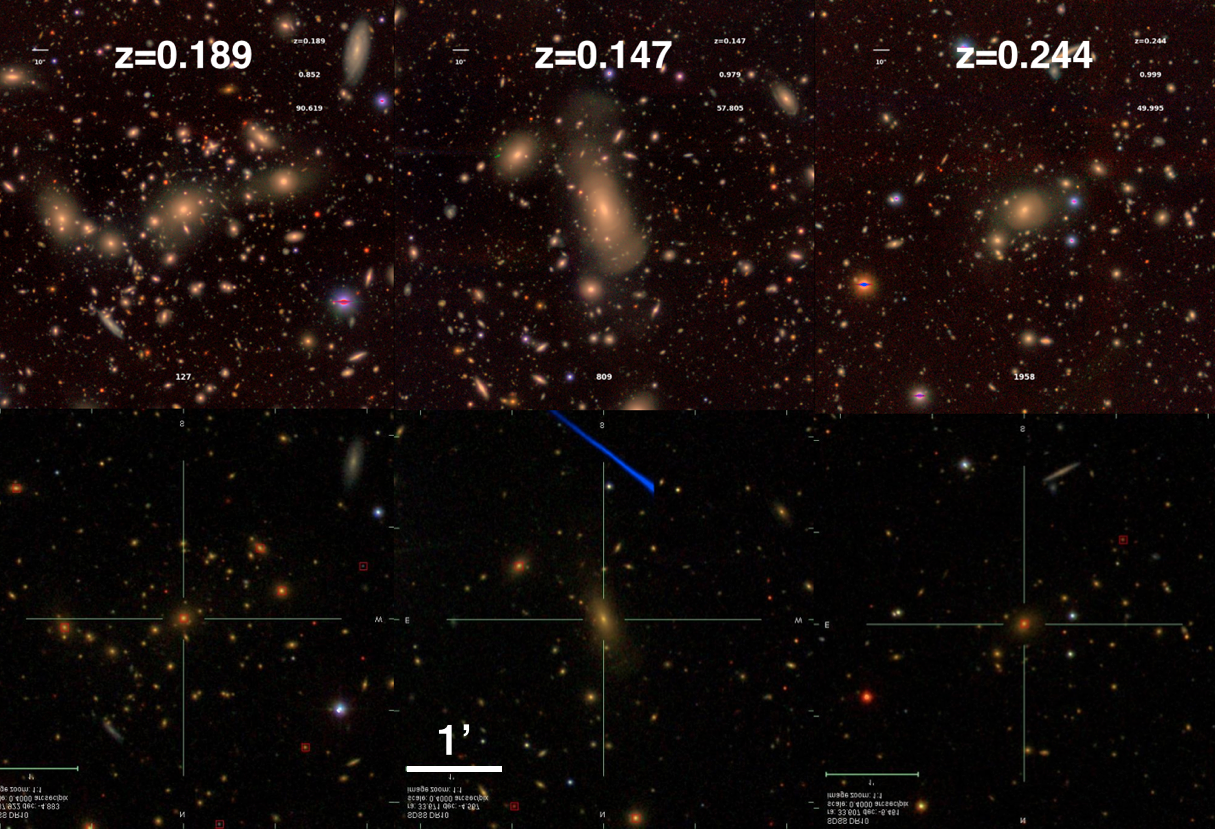
\includegraphics[width=15.5cm]{fig/fig1.png}
    \caption{Figure.1\todo{Caption}}\label{figure:1}
\end{figure}

% Fig. 2
\clearpage
\figurenum{2a}
\begin{figure}
    \centering 
    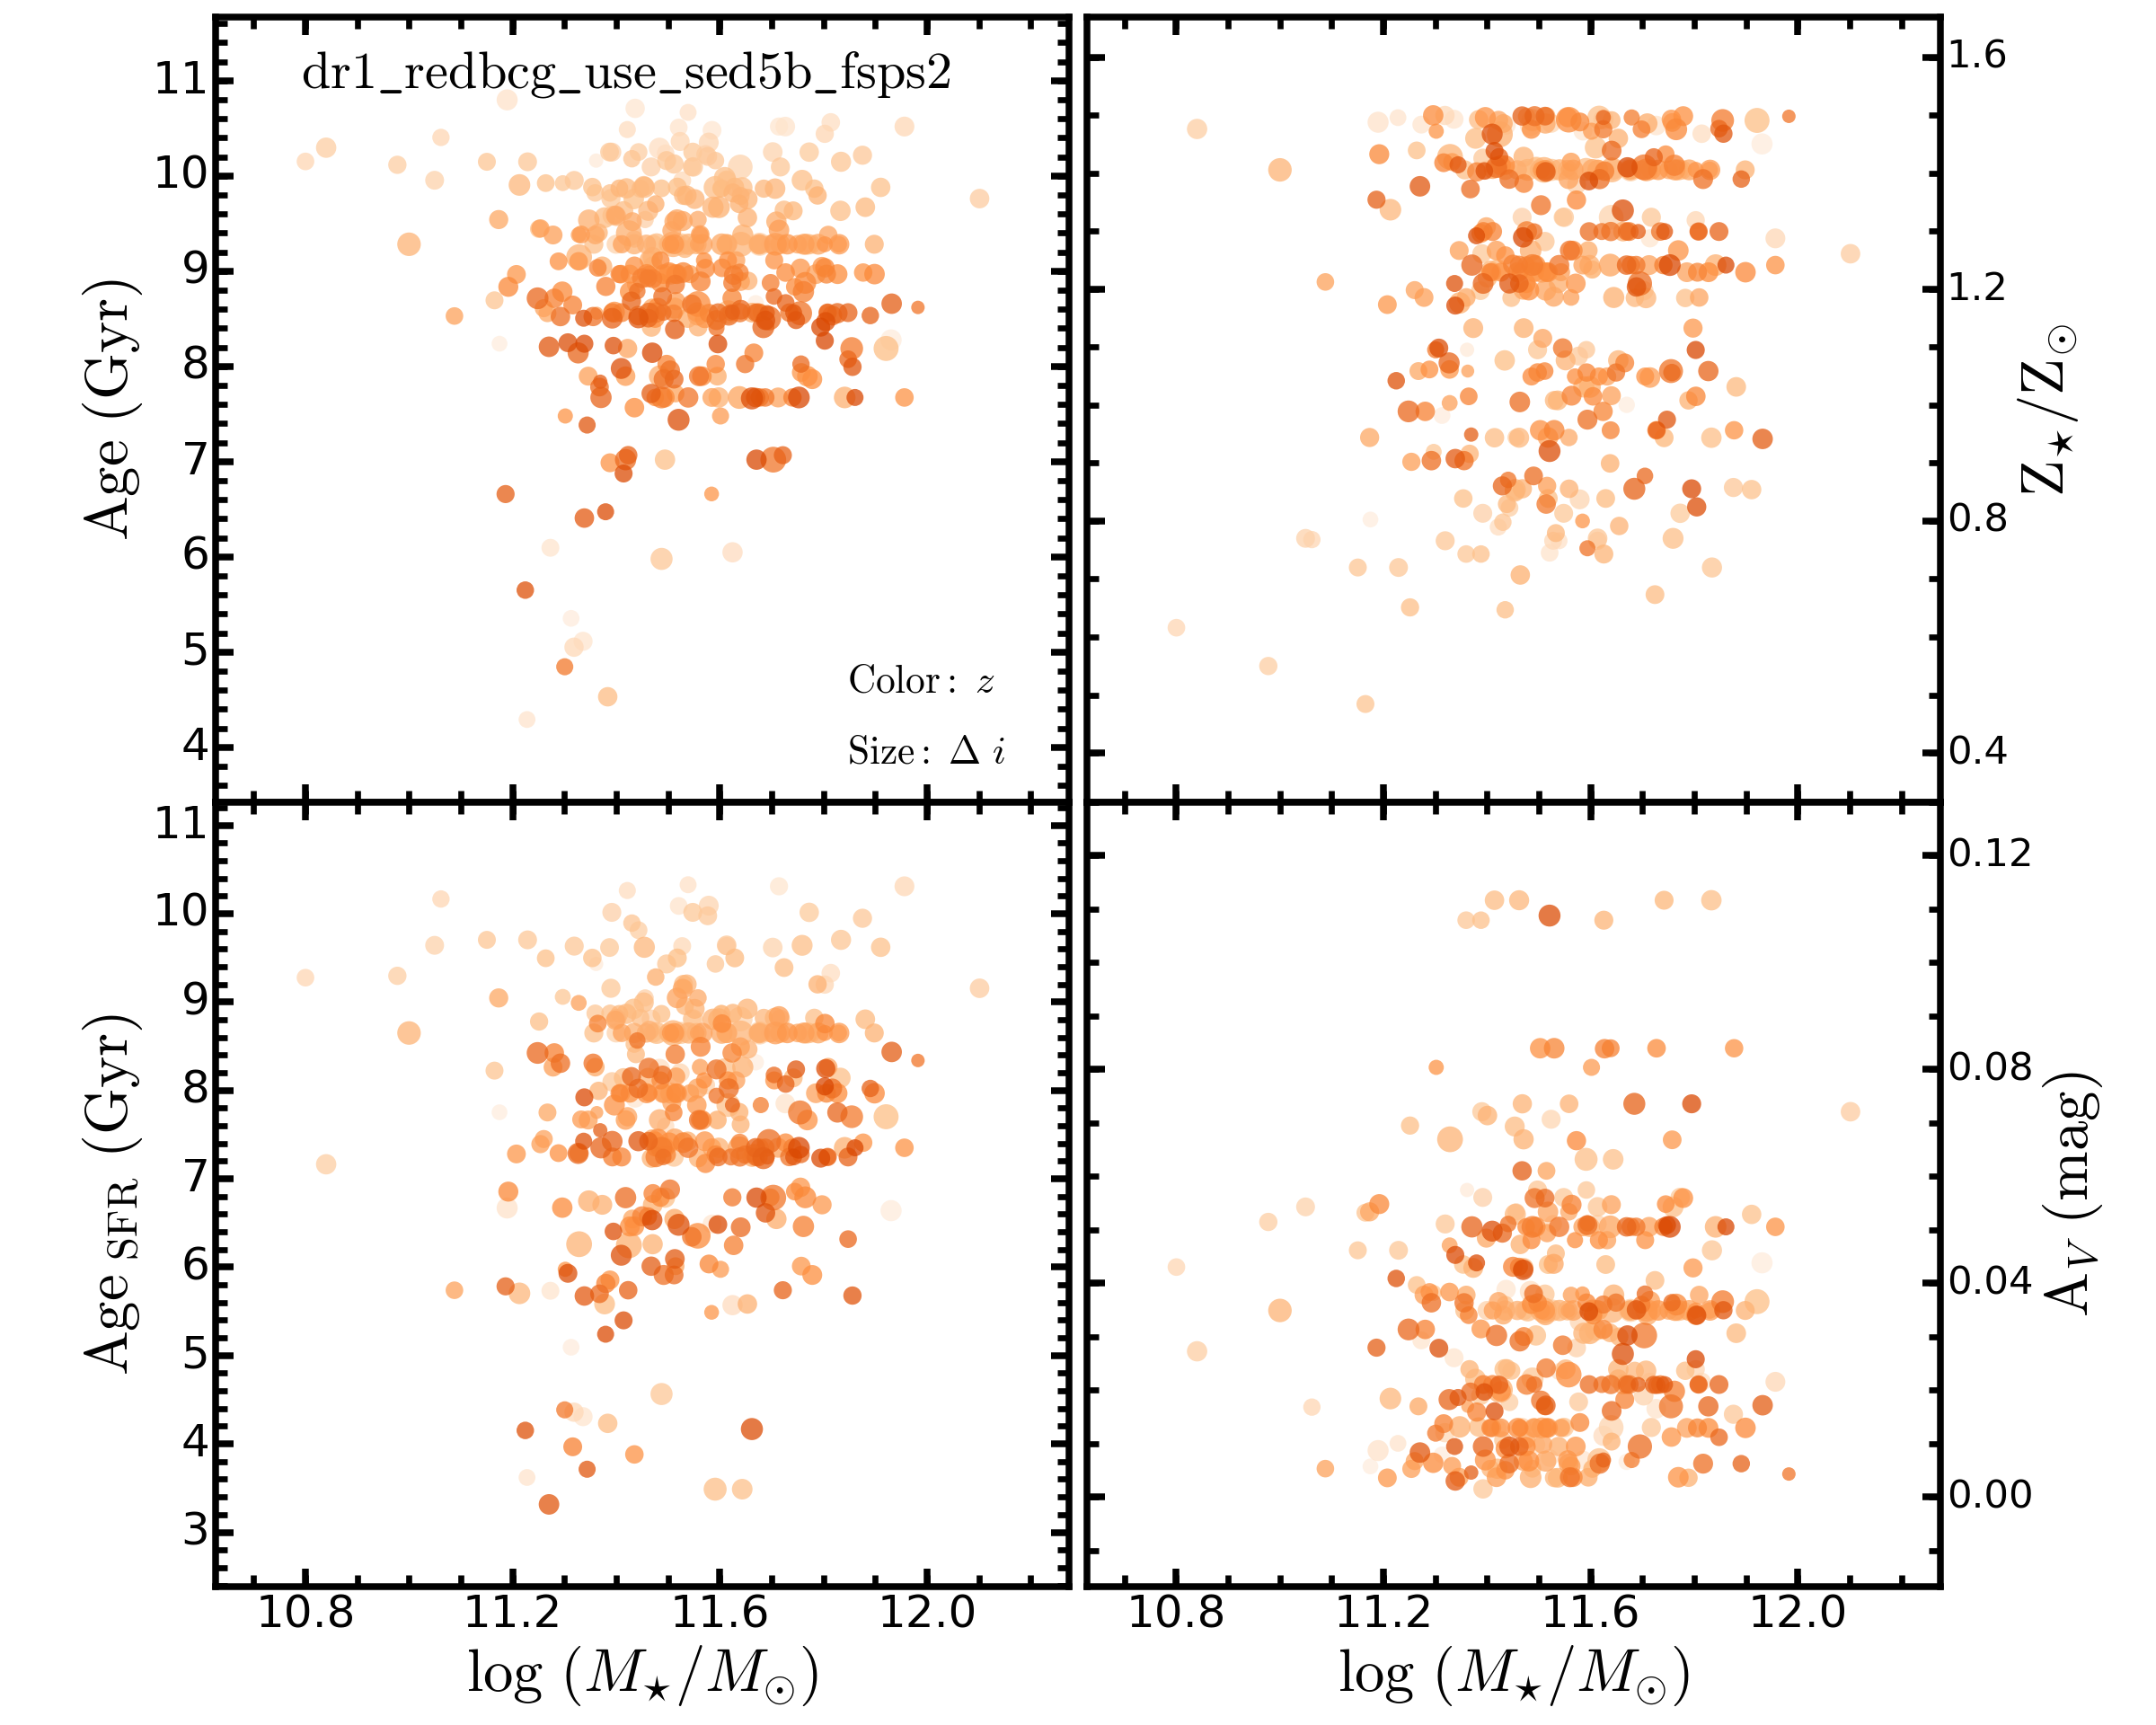
\includegraphics[width=11.5cm]{fig/dr1_redbcg_use_sed5b_fsps2_logm_plots}
    \caption{Figure.2a\todo{Caption}}\label{figure:2a}
\end{figure}

\figurenum{2b}
\begin{figure}
    \centering 
    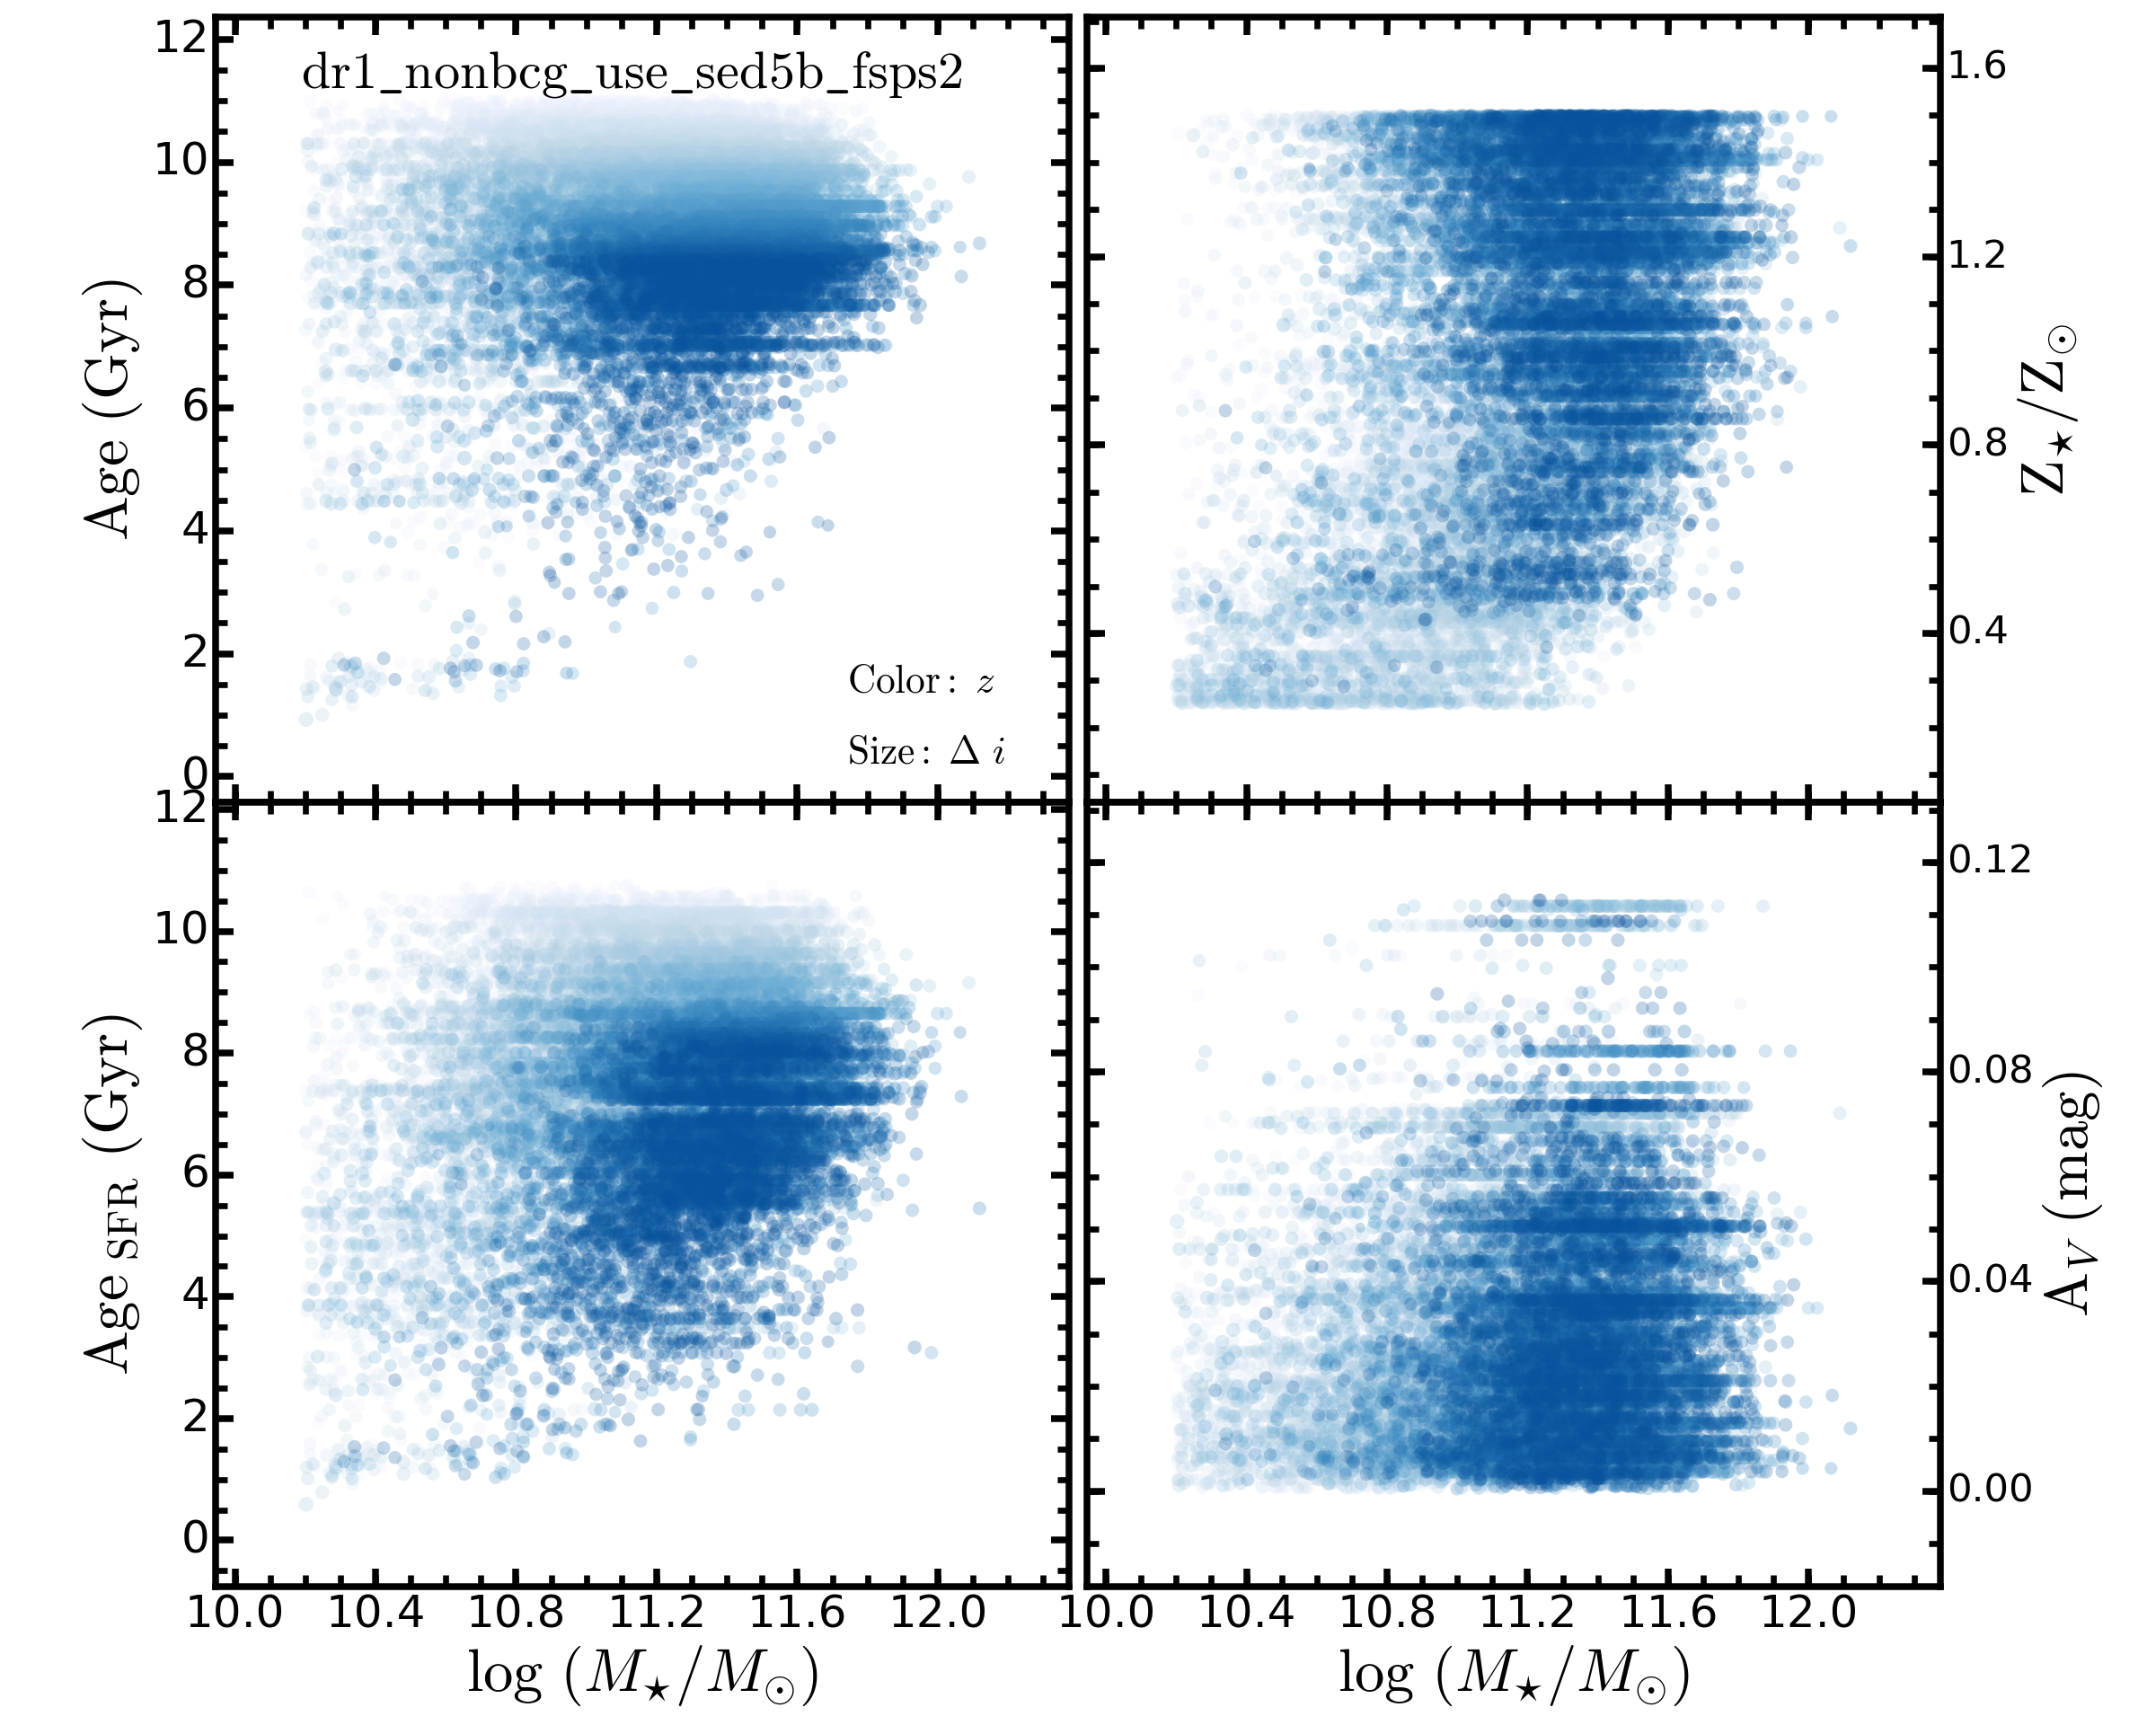
\includegraphics[width=11.5cm]{fig/dr1_nonbcg_use_sed5b_fsps2_logm_plots}
    \caption{Figure.2b\todo{Caption}}\label{figure:2b}
\end{figure}

% Fig. 3
\clearpage
\figurenum{3a}
\begin{figure}
    \centering 
    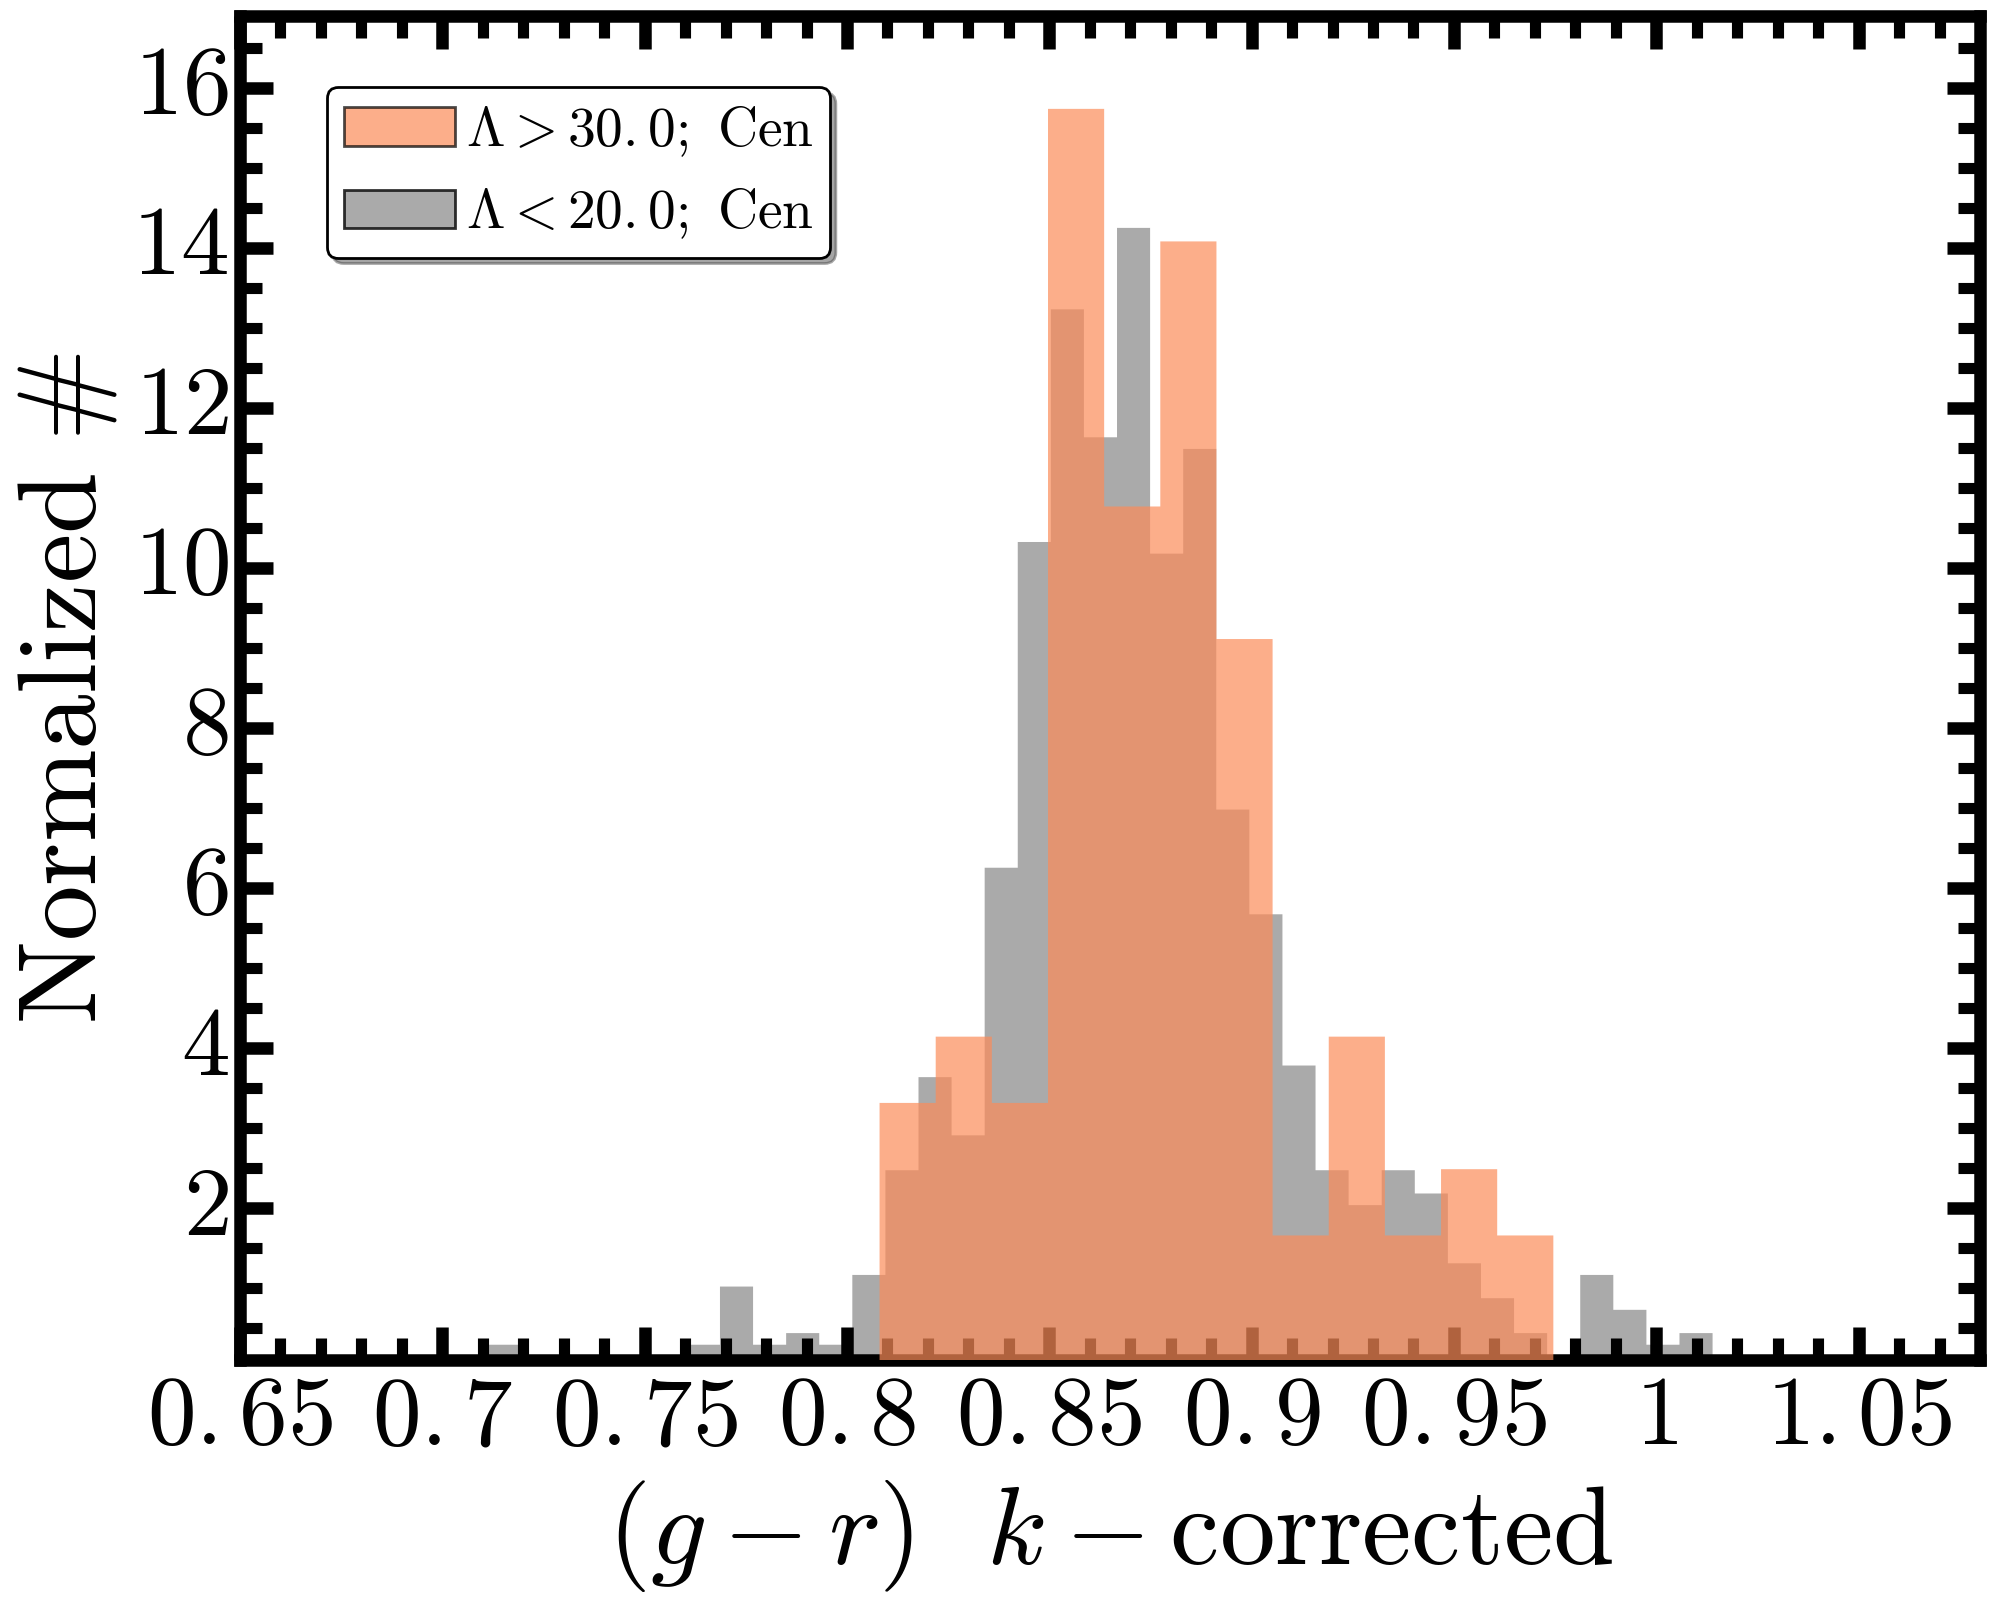
\includegraphics[width=10.5cm]{fig/dr1_redbcg_isedfit_mass_fsps1_sbpsum_imgsub_use_grKcor_hist}
    \caption{Figure.3a\todo{Caption}}\label{figure:3a}
\end{figure}

\figurenum{3b}
\begin{figure}
    \centering 
    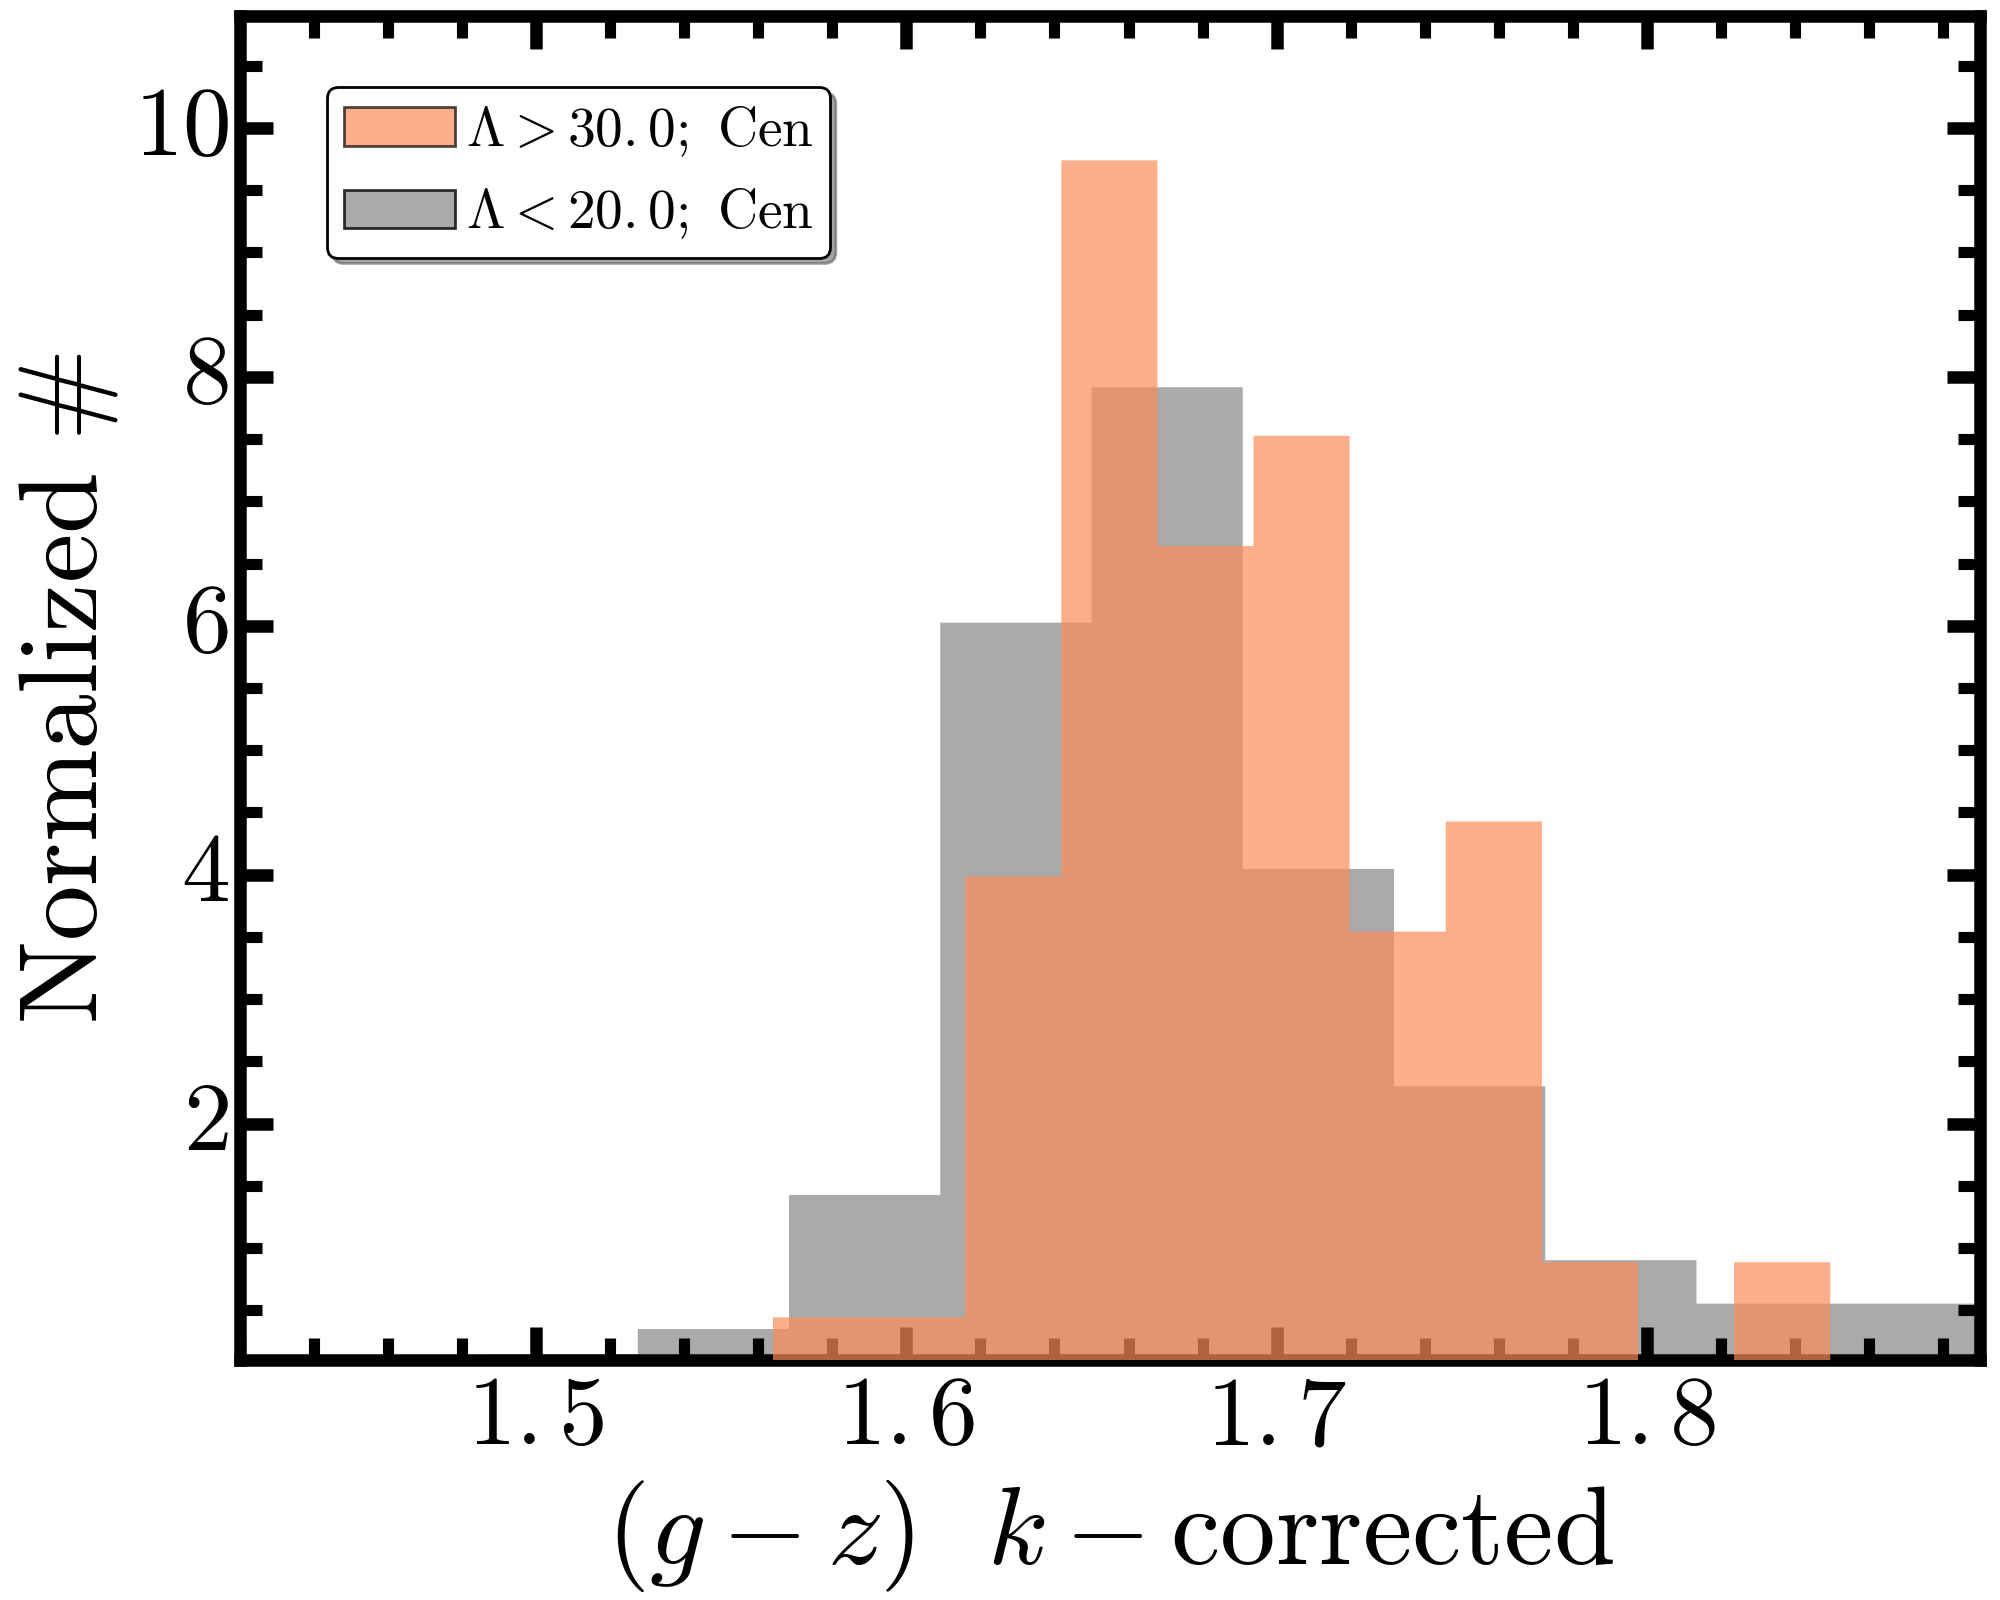
\includegraphics[width=10.5cm]{fig/dr1_redbcg_isedfit_mass_fsps1_sbpsum_imgsub_use_gzKcor_hist}
    \caption{Figure.3b\todo{Caption}}\label{figure:3b}
\end{figure}

\figurenum{3c}
\begin{figure}
    \centering 
    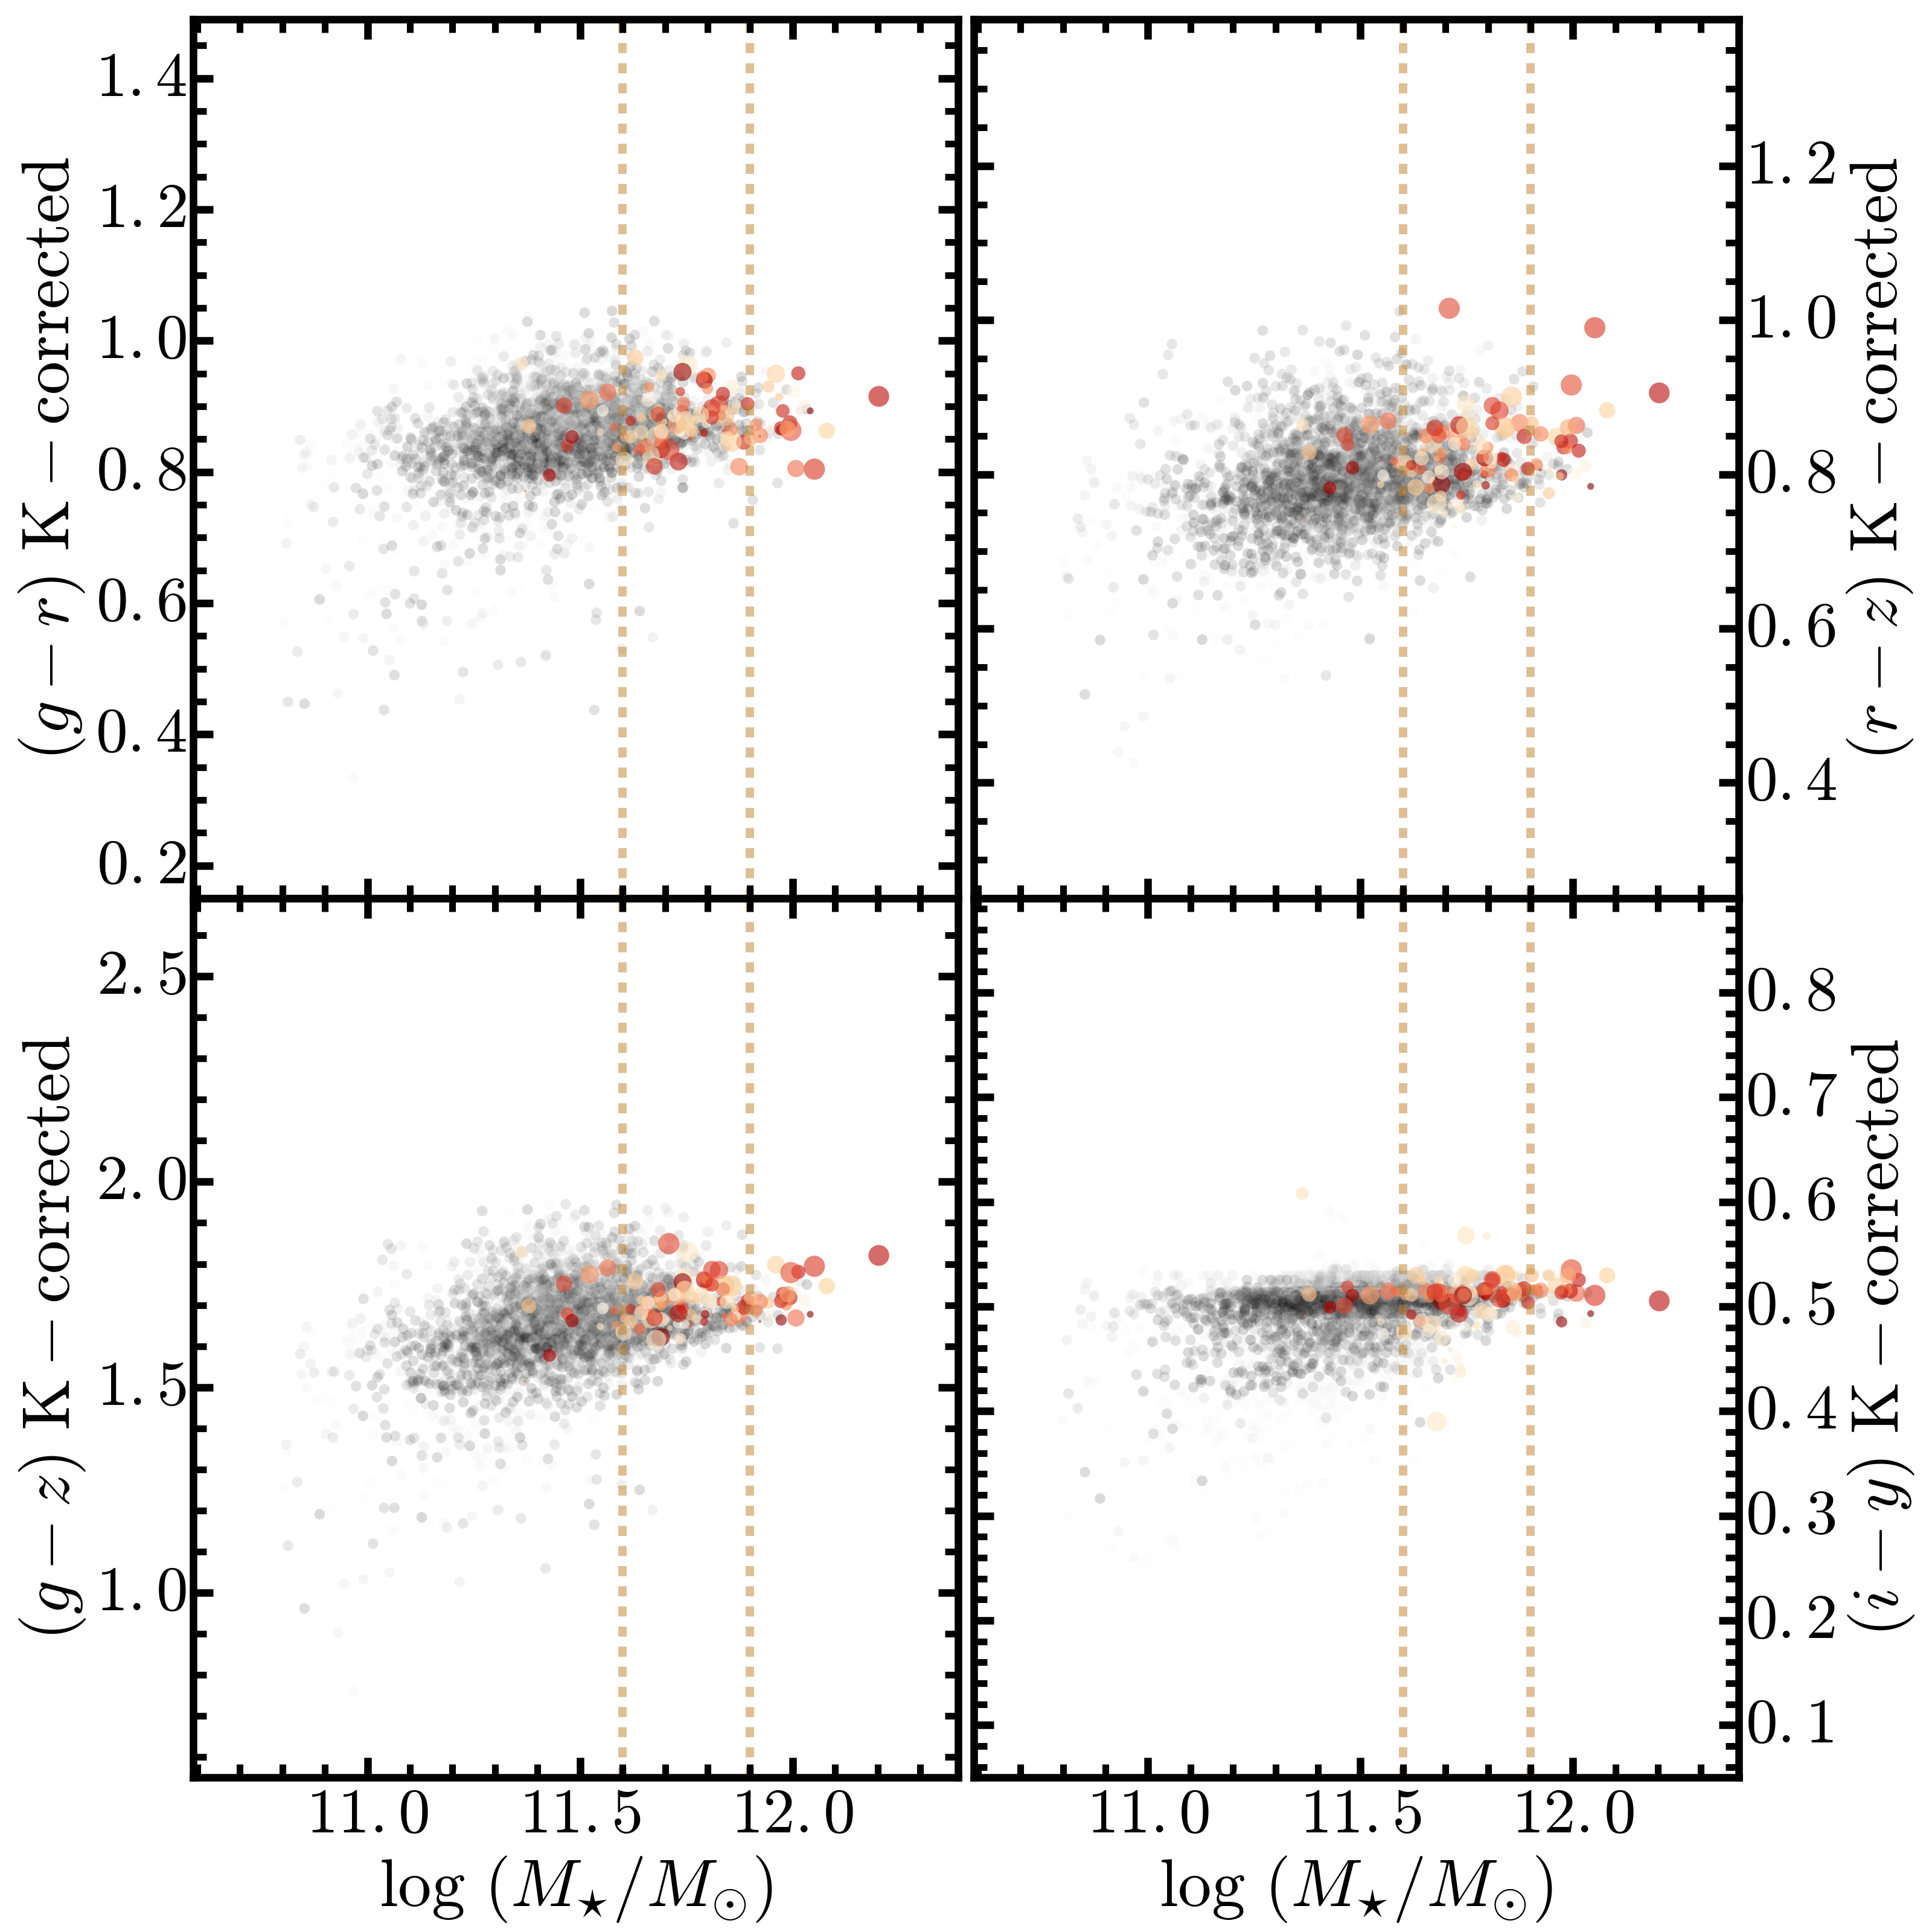
\includegraphics[width=12.5cm]{fig/dr1_redbcg_isedfit_mass_fsps1_sbpsum_imgsub_use_mass_color}
    \caption{Figure.3c\todo{Caption}}\label{figure:3c}
\end{figure}

% Fig. 4
\clearpage
\figurenum{4}
\begin{figure}
    \centering 
    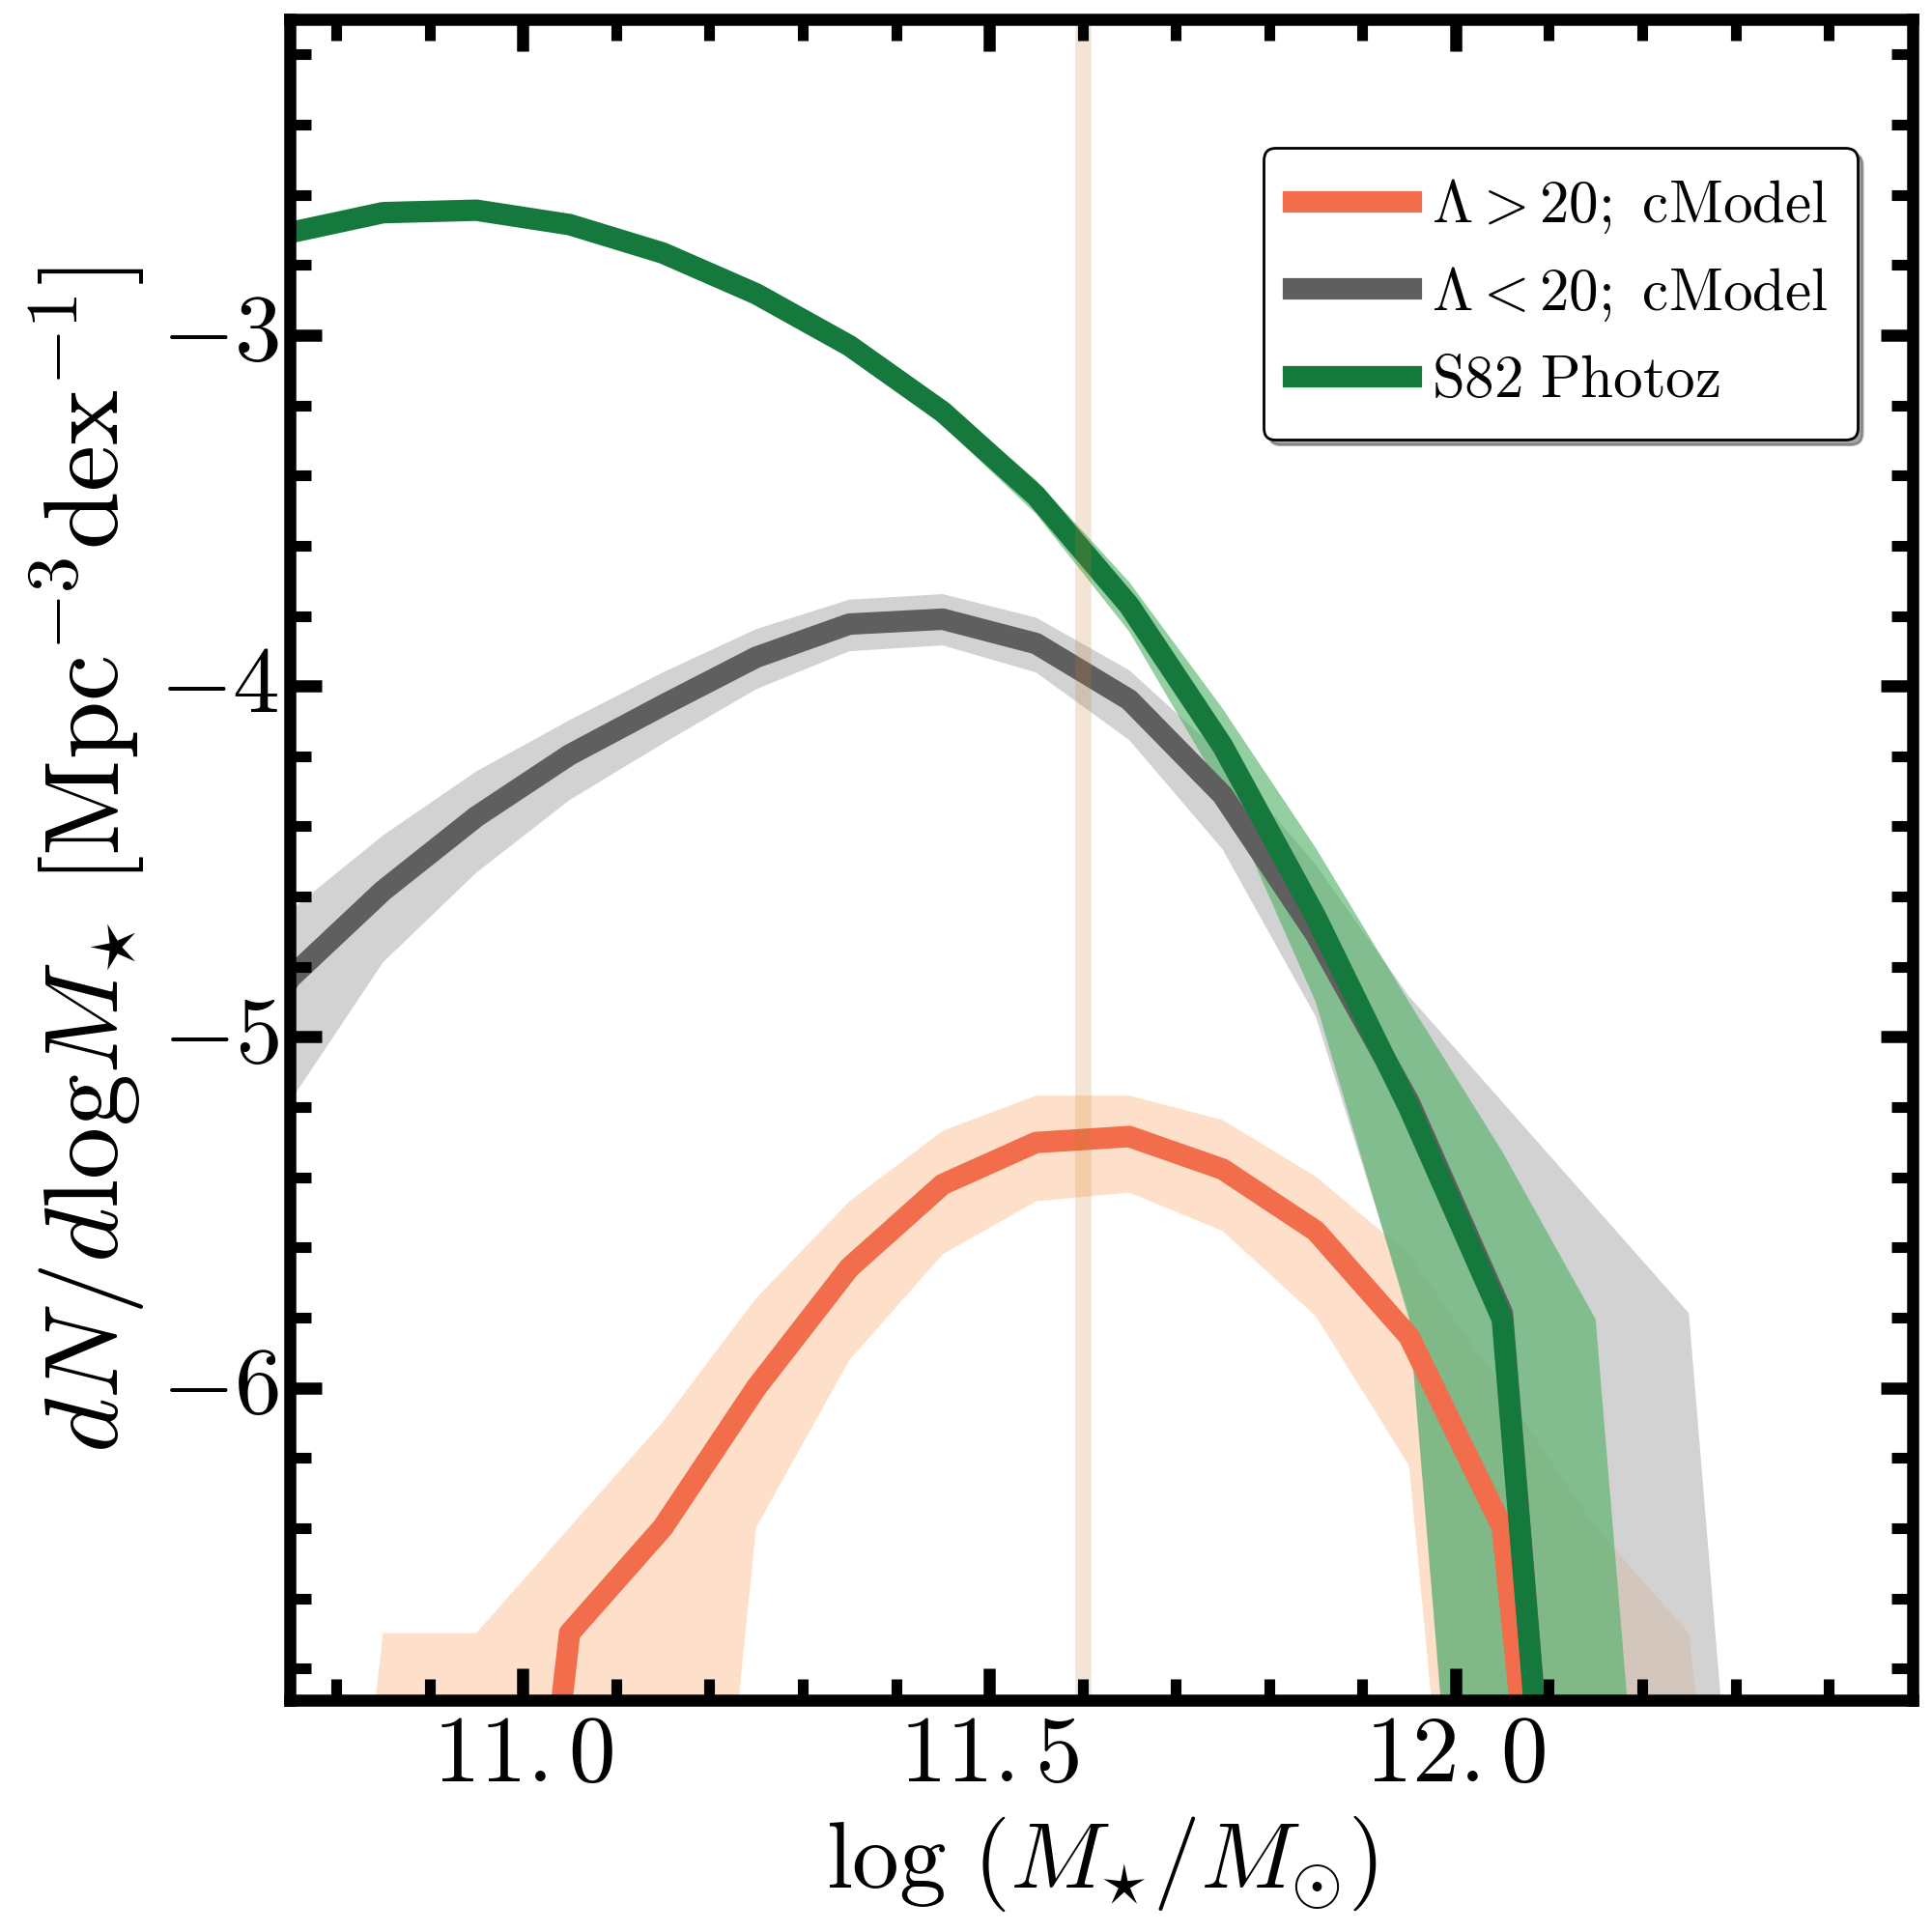
\includegraphics[width=14.5cm]{fig/dr1_redbcg_isedfit_mass_fsps1_sbpsum_imgsub_use_logm_distribution_s82}
    \caption{Figure.4\todo{Caption}}\label{figure:4}
\end{figure}

% Fig. 5
\clearpage
\figurenum{5}
\begin{figure}
    \centering 
    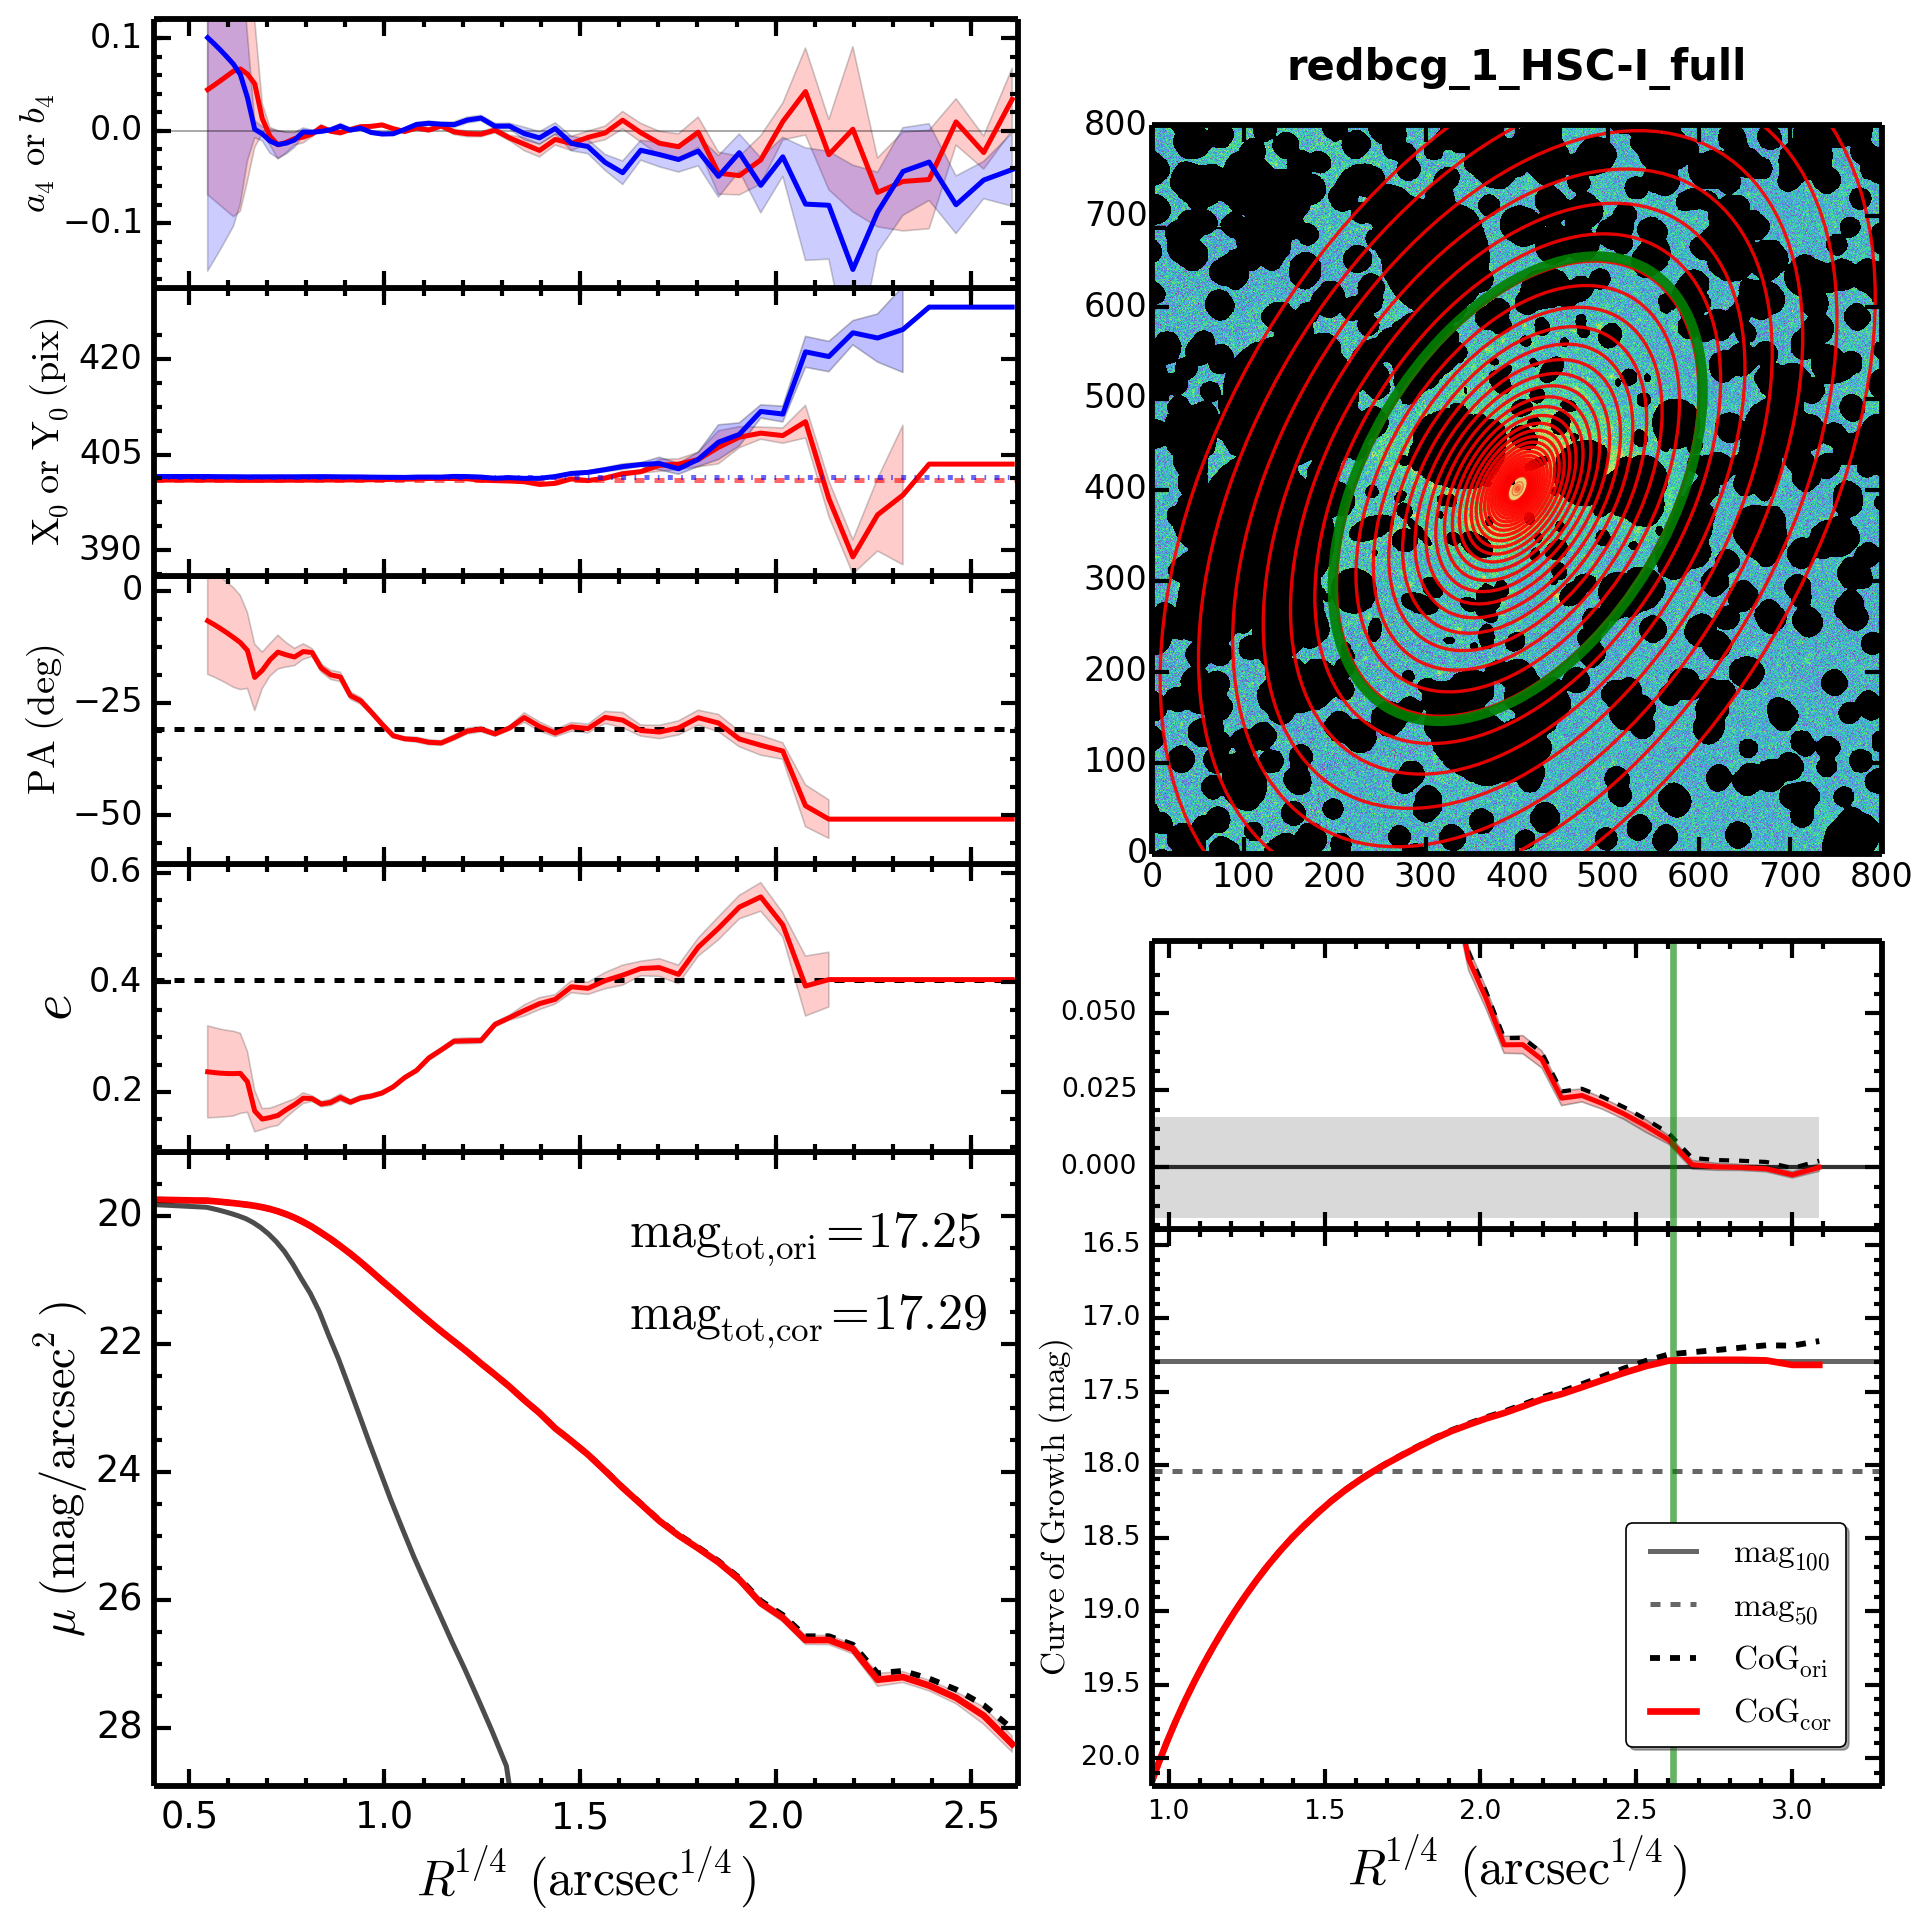
\includegraphics[width=15.5cm]{fig/redbcg_1_HSC-I_full_imgsub_ellip_default_sum.png}
    \caption{Figure.5\todo{Caption}}\label{figure:5}
\end{figure}

% Fig. 6
\clearpage
\figurenum{6}
\begin{figure}
    \centering 
    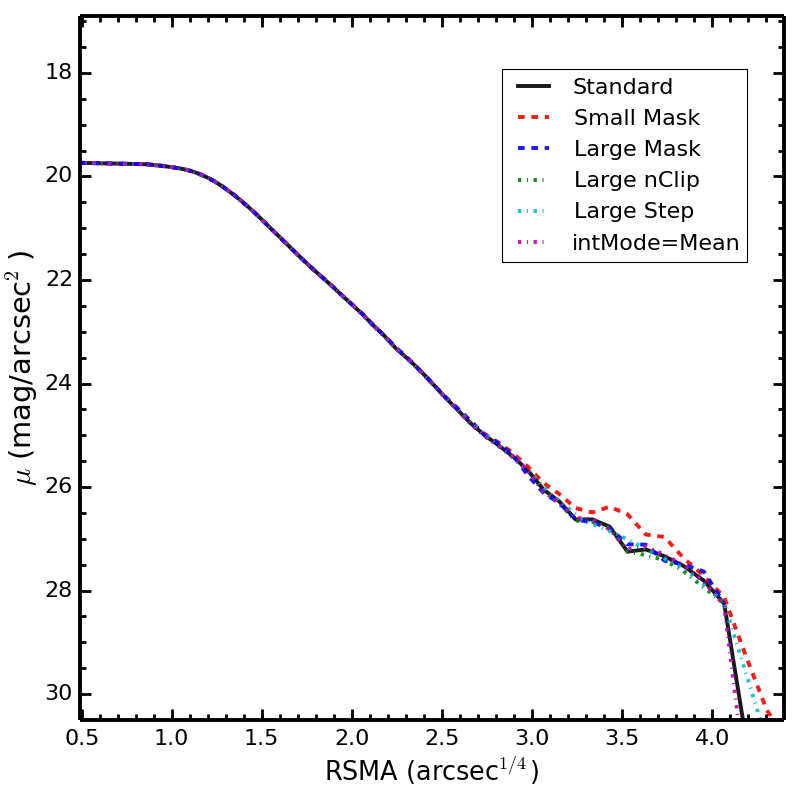
\includegraphics[width=14.0cm]{fig/redbcg_1_HSC-I_full_imgsub_ellip_default_compare.png}
    \caption{Figure.6\todo{Caption}}\label{figure:6}
\end{figure}

%%%%%%%%%%%%: End of the File %%%%%%%%%%%%

\end{CJK*}

\clearpage 

%%%%%%%%%%%: Possible Tables %%%%%%%%%%%%%
%\begin{deluxetable}{c ccc cc cc}[b!]
\tabletypesize{\scriptsize}
\tablewidth{0pt}
\tablecolumns{8}
\tablenum{1}
\tablecaption{Average \mden{} Profiles of Massive Galaxies in Different Stellar Mass Bins}
%% ------------------------------------------------------------------------------------ %% 
\tablehead{
    \colhead{Radius} & 
    \multicolumn{3}{c}{[\mden{}]; Combined samples} &
    \multicolumn{2}{c}{[\mden{}]; $M_{\star,100\ \mathrm{kpc}}$-matched} &
    \multicolumn{2}{c}{[\mden{}]; $M_{\star,10\ \mathrm{kpc}}$-matched}
	\vspace{1.4ex}
    %------------------------------------------------------------------------------------%
    \nl 
    \colhead{kpc} & 
    \multicolumn{3}{c}{$\log (M_{\odot}/\mathrm{kpc}^2)$} &
    \multicolumn{2}{c}{$\log (M_{\odot}/\mathrm{kpc}^2)$} &
    \multicolumn{2}{c}{$\log (M_{\odot}/\mathrm{kpc}^2)$}
	\vspace{1.4ex}
    %------------------------------------------------------------------------------------%
    \nl 
    \colhead{} & 
    \colhead{$\log \frac{M_{\star,100\mathrm{kpc}}}{M_{\odot}}\in$[11.4, 11.6]} & 
    \colhead{[11.6, 11.8]} & 
    \colhead{[11.8, 12.0]}\hspace{2.0ex} & 
    \colhead{\texttt{cenHighMh}} & 
    \colhead{\texttt{cenLowMh}} & 
    \colhead{\texttt{cenHighMh}}\hspace{2.0ex} & 
    \colhead{\texttt{cenLowMh}}
    %------------------------------------------------------------------------------------%
	\vspace{1.6ex}
    %------------------------------------------------------------------------------------%
    \nl
    \colhead{    (1)} &
    \colhead{    (2)} &
    \colhead{    (3)} &
    \colhead{    (4)} &
    \colhead{    (5)} &
    \colhead{    (6)} &
    \colhead{    (7)} &
    \colhead{    (8)}
    %------------------------------------------------------------------------------------%
}
%% ------------------------------------------------------------------------------------ %% 
\startdata
%% ------------------------------------------------------------------------------------ %% 

0.0 & $ 9.23\substack{+0.00 \\ -0.00}$ &$ 9.31\substack{+0.00 \\ -0.01}$ &$ 9.32\substack{+0.01 \\ -0.01}$ &$ 9.31\substack{+0.02 \\ -0.02}$ &$ 9.34\substack{+0.01 \\ -0.01}$ &$ 9.31\substack{+0.02 \\ -0.02}$ &$ 9.34\substack{+0.02 \\ -0.02}$ \\
 0.6 & $ 9.20\substack{+0.00 \\ -0.00}$ &$ 9.28\substack{+0.00 \\ -0.01}$ &$ 9.29\substack{+0.01 \\ -0.01}$ &$ 9.27\substack{+0.02 \\ -0.02}$ &$ 9.31\substack{+0.01 \\ -0.01}$ &$ 9.28\substack{+0.02 \\ -0.02}$ &$ 9.31\substack{+0.02 \\ -0.02}$ \\
 1.0 & $ 9.16\substack{+0.00 \\ -0.00}$ &$ 9.24\substack{+0.00 \\ -0.00}$ &$ 9.26\substack{+0.01 \\ -0.01}$ &$ 9.24\substack{+0.02 \\ -0.02}$ &$ 9.27\substack{+0.01 \\ -0.01}$ &$ 9.25\substack{+0.02 \\ -0.02}$ &$ 9.27\substack{+0.02 \\ -0.02}$ \\
 1.4 & $ 9.12\substack{+0.00 \\ -0.00}$ &$ 9.20\substack{+0.00 \\ -0.00}$ &$ 9.23\substack{+0.01 \\ -0.01}$ &$ 9.20\substack{+0.02 \\ -0.02}$ &$ 9.23\substack{+0.01 \\ -0.01}$ &$ 9.21\substack{+0.02 \\ -0.01}$ &$ 9.23\substack{+0.02 \\ -0.01}$ \\
 1.7 & $ 9.06\substack{+0.00 \\ -0.00}$ &$ 9.15\substack{+0.00 \\ -0.00}$ &$ 9.19\substack{+0.01 \\ -0.01}$ &$ 9.15\substack{+0.02 \\ -0.02}$ &$ 9.19\substack{+0.01 \\ -0.01}$ &$ 9.16\substack{+0.01 \\ -0.01}$ &$ 9.18\substack{+0.01 \\ -0.01}$ \\
 2.0 & $ 9.00\substack{+0.00 \\ -0.00}$ &$ 9.10\substack{+0.00 \\ -0.00}$ &$ 9.15\substack{+0.01 \\ -0.01}$ &$ 9.09\substack{+0.01 \\ -0.02}$ &$ 9.13\substack{+0.01 \\ -0.01}$ &$ 9.11\substack{+0.01 \\ -0.01}$ &$ 9.12\substack{+0.01 \\ -0.01}$ \\
 2.4 & $ 8.93\substack{+0.00 \\ -0.00}$ &$ 9.03\substack{+0.00 \\ -0.00}$ &$ 9.09\substack{+0.01 \\ -0.01}$ &$ 9.03\substack{+0.02 \\ -0.02}$ &$ 9.07\substack{+0.01 \\ -0.01}$ &$ 9.05\substack{+0.01 \\ -0.01}$ &$ 9.05\substack{+0.01 \\ -0.01}$ \\
 2.7 & $ 8.87\substack{+0.00 \\ -0.00}$ &$ 8.97\substack{+0.00 \\ -0.00}$ &$ 9.04\substack{+0.01 \\ -0.01}$ &$ 8.97\substack{+0.01 \\ -0.01}$ &$ 9.01\substack{+0.01 \\ -0.01}$ &$ 9.00\substack{+0.01 \\ -0.01}$ &$ 8.99\substack{+0.01 \\ -0.01}$ \\
 3.0 & $ 8.80\substack{+0.00 \\ -0.00}$ &$ 8.90\substack{+0.00 \\ -0.00}$ &$ 8.98\substack{+0.01 \\ -0.01}$ &$ 8.90\substack{+0.01 \\ -0.01}$ &$ 8.95\substack{+0.01 \\ -0.01}$ &$ 8.93\substack{+0.01 \\ -0.01}$ &$ 8.92\substack{+0.01 \\ -0.01}$ \\
 3.4 & $ 8.72\substack{+0.00 \\ -0.00}$ &$ 8.83\substack{+0.00 \\ -0.00}$ &$ 8.92\substack{+0.01 \\ -0.01}$ &$ 8.83\substack{+0.01 \\ -0.01}$ &$ 8.88\substack{+0.01 \\ -0.01}$ &$ 8.86\substack{+0.01 \\ -0.01}$ &$ 8.85\substack{+0.01 \\ -0.01}$ \\
 3.7 & $ 8.66\substack{+0.00 \\ -0.00}$ &$ 8.78\substack{+0.00 \\ -0.00}$ &$ 8.87\substack{+0.01 \\ -0.01}$ &$ 8.78\substack{+0.01 \\ -0.01}$ &$ 8.83\substack{+0.01 \\ -0.01}$ &$ 8.81\substack{+0.01 \\ -0.01}$ &$ 8.79\substack{+0.01 \\ -0.01}$ \\
 4.1 & $ 8.60\substack{+0.00 \\ -0.00}$ &$ 8.72\substack{+0.00 \\ -0.00}$ &$ 8.82\substack{+0.01 \\ -0.01}$ &$ 8.72\substack{+0.01 \\ -0.01}$ &$ 8.77\substack{+0.01 \\ -0.01}$ &$ 8.76\substack{+0.01 \\ -0.01}$ &$ 8.73\substack{+0.01 \\ -0.01}$ \\
 4.4 & $ 8.54\substack{+0.00 \\ -0.00}$ &$ 8.66\substack{+0.00 \\ -0.00}$ &$ 8.77\substack{+0.01 \\ -0.01}$ &$ 8.66\substack{+0.01 \\ -0.01}$ &$ 8.72\substack{+0.01 \\ -0.01}$ &$ 8.70\substack{+0.01 \\ -0.01}$ &$ 8.67\substack{+0.01 \\ -0.01}$ \\
 4.8 & $ 8.48\substack{+0.00 \\ -0.00}$ &$ 8.60\substack{+0.00 \\ -0.00}$ &$ 8.71\substack{+0.01 \\ -0.01}$ &$ 8.60\substack{+0.01 \\ -0.01}$ &$ 8.66\substack{+0.01 \\ -0.01}$ &$ 8.65\substack{+0.01 \\ -0.01}$ &$ 8.61\substack{+0.01 \\ -0.01}$ \\
 6.2 & $ 8.26\substack{+0.00 \\ -0.00}$ &$ 8.40\substack{+0.00 \\ -0.00}$ &$ 8.53\substack{+0.01 \\ -0.01}$ &$ 8.41\substack{+0.01 \\ -0.01}$ &$ 8.46\substack{+0.01 \\ -0.01}$ &$ 8.46\substack{+0.02 \\ -0.02}$ &$ 8.40\substack{+0.02 \\ -0.02}$ \\
 7.6 & $ 8.09\substack{+0.00 \\ -0.00}$ &$ 8.24\substack{+0.00 \\ -0.00}$ &$ 8.39\substack{+0.01 \\ -0.01}$ &$ 8.27\substack{+0.01 \\ -0.01}$ &$ 8.31\substack{+0.01 \\ -0.01}$ &$ 8.31\substack{+0.02 \\ -0.02}$ &$ 8.23\substack{+0.02 \\ -0.02}$ \\
 9.0 & $ 7.95\substack{+0.00 \\ -0.00}$ &$ 8.10\substack{+0.00 \\ -0.00}$ &$ 8.27\substack{+0.01 \\ -0.01}$ &$ 8.14\substack{+0.02 \\ -0.02}$ &$ 8.18\substack{+0.01 \\ -0.01}$ &$ 8.19\substack{+0.02 \\ -0.02}$ &$ 8.09\substack{+0.02 \\ -0.02}$ \\
10.3 & $ 7.82\substack{+0.00 \\ -0.00}$ &$ 7.99\substack{+0.00 \\ -0.00}$ &$ 8.16\substack{+0.01 \\ -0.01}$ &$ 8.03\substack{+0.02 \\ -0.01}$ &$ 8.06\substack{+0.01 \\ -0.01}$ &$ 8.09\substack{+0.02 \\ -0.02}$ &$ 7.97\substack{+0.02 \\ -0.02}$ \\
11.7 & $ 7.70\substack{+0.00 \\ -0.00}$ &$ 7.88\substack{+0.00 \\ -0.00}$ &$ 8.06\substack{+0.01 \\ -0.01}$ &$ 7.93\substack{+0.02 \\ -0.02}$ &$ 7.96\substack{+0.01 \\ -0.01}$ &$ 7.99\substack{+0.02 \\ -0.02}$ &$ 7.85\substack{+0.02 \\ -0.02}$ \\
13.0 & $ 7.60\substack{+0.00 \\ -0.00}$ &$ 7.78\substack{+0.00 \\ -0.00}$ &$ 7.98\substack{+0.01 \\ -0.01}$ &$ 7.85\substack{+0.02 \\ -0.02}$ &$ 7.87\substack{+0.01 \\ -0.01}$ &$ 7.90\substack{+0.02 \\ -0.02}$ &$ 7.75\substack{+0.02 \\ -0.02}$ \\
14.5 & $ 7.50\substack{+0.00 \\ -0.00}$ &$ 7.69\substack{+0.00 \\ -0.00}$ &$ 7.90\substack{+0.01 \\ -0.01}$ &$ 7.76\substack{+0.02 \\ -0.02}$ &$ 7.78\substack{+0.01 \\ -0.01}$ &$ 7.82\substack{+0.02 \\ -0.02}$ &$ 7.65\substack{+0.02 \\ -0.02}$ \\
16.0 & $ 7.39\substack{+0.00 \\ -0.00}$ &$ 7.60\substack{+0.00 \\ -0.00}$ &$ 7.82\substack{+0.01 \\ -0.01}$ &$ 7.68\substack{+0.02 \\ -0.02}$ &$ 7.69\substack{+0.01 \\ -0.01}$ &$ 7.74\substack{+0.02 \\ -0.03}$ &$ 7.56\substack{+0.02 \\ -0.03}$ \\
17.3 & $ 7.31\substack{+0.00 \\ -0.00}$ &$ 7.52\substack{+0.00 \\ -0.00}$ &$ 7.76\substack{+0.01 \\ -0.01}$ &$ 7.61\substack{+0.02 \\ -0.02}$ &$ 7.62\substack{+0.01 \\ -0.01}$ &$ 7.67\substack{+0.03 \\ -0.03}$ &$ 7.48\substack{+0.03 \\ -0.03}$ \\
18.7 & $ 7.23\substack{+0.00 \\ -0.00}$ &$ 7.45\substack{+0.00 \\ -0.00}$ &$ 7.69\substack{+0.01 \\ -0.01}$ &$ 7.55\substack{+0.02 \\ -0.02}$ &$ 7.55\substack{+0.01 \\ -0.01}$ &$ 7.61\substack{+0.03 \\ -0.03}$ &$ 7.40\substack{+0.03 \\ -0.03}$ \\
22.6 & $ 7.02\substack{+0.00 \\ -0.00}$ &$ 7.27\substack{+0.00 \\ -0.00}$ &$ 7.54\substack{+0.01 \\ -0.01}$ &$ 7.38\substack{+0.02 \\ -0.02}$ &$ 7.37\substack{+0.01 \\ -0.01}$ &$ 7.45\substack{+0.03 \\ -0.03}$ &$ 7.21\substack{+0.03 \\ -0.03}$ \\
26.1 & $ 6.86\substack{+0.00 \\ -0.00}$ &$ 7.12\substack{+0.00 \\ -0.00}$ &$ 7.41\substack{+0.01 \\ -0.01}$ &$ 7.25\substack{+0.02 \\ -0.02}$ &$ 7.24\substack{+0.01 \\ -0.01}$ &$ 7.32\substack{+0.03 \\ -0.03}$ &$ 7.05\substack{+0.03 \\ -0.03}$ \\
30.0 & $ 6.70\substack{+0.00 \\ -0.00}$ &$ 6.98\substack{+0.00 \\ -0.00}$ &$ 7.29\substack{+0.01 \\ -0.01}$ &$ 7.13\substack{+0.03 \\ -0.02}$ &$ 7.10\substack{+0.01 \\ -0.01}$ &$ 7.20\substack{+0.03 \\ -0.04}$ &$ 6.90\substack{+0.03 \\ -0.04}$ \\
33.7 & $ 6.55\substack{+0.00 \\ -0.00}$ &$ 6.85\substack{+0.01 \\ -0.01}$ &$ 7.18\substack{+0.01 \\ -0.01}$ &$ 7.01\substack{+0.03 \\ -0.03}$ &$ 6.98\substack{+0.01 \\ -0.01}$ &$ 7.09\substack{+0.03 \\ -0.03}$ &$ 6.76\substack{+0.03 \\ -0.03}$ \\
37.8 & $ 6.41\substack{+0.00 \\ -0.00}$ &$ 6.72\substack{+0.01 \\ -0.01}$ &$ 7.07\substack{+0.01 \\ -0.01}$ &$ 6.90\substack{+0.03 \\ -0.03}$ &$ 6.85\substack{+0.01 \\ -0.01}$ &$ 6.98\substack{+0.04 \\ -0.04}$ &$ 6.63\substack{+0.04 \\ -0.04}$ \\
41.6 & $ 6.29\substack{+0.01 \\ -0.01}$ &$ 6.61\substack{+0.01 \\ -0.01}$ &$ 6.98\substack{+0.01 \\ -0.01}$ &$ 6.81\substack{+0.03 \\ -0.03}$ &$ 6.75\substack{+0.01 \\ -0.01}$ &$ 6.89\substack{+0.04 \\ -0.04}$ &$ 6.51\substack{+0.04 \\ -0.04}$ \\
45.7 & $ 6.17\substack{+0.01 \\ -0.01}$ &$ 6.50\substack{+0.01 \\ -0.01}$ &$ 6.88\substack{+0.01 \\ -0.01}$ &$ 6.71\substack{+0.03 \\ -0.03}$ &$ 6.64\substack{+0.01 \\ -0.01}$ &$ 6.79\substack{+0.04 \\ -0.04}$ &$ 6.39\substack{+0.04 \\ -0.04}$ \\
49.3 & $ 6.07\substack{+0.01 \\ -0.01}$ &$ 6.41\substack{+0.01 \\ -0.01}$ &$ 6.80\substack{+0.01 \\ -0.02}$ &$ 6.62\substack{+0.03 \\ -0.03}$ &$ 6.56\substack{+0.01 \\ -0.01}$ &$ 6.70\substack{+0.04 \\ -0.04}$ &$ 6.30\substack{+0.04 \\ -0.04}$ \\
53.1 & $ 5.98\substack{+0.01 \\ -0.01}$ &$ 6.33\substack{+0.01 \\ -0.01}$ &$ 6.71\substack{+0.02 \\ -0.02}$ &$ 6.55\substack{+0.03 \\ -0.03}$ &$ 6.46\substack{+0.01 \\ -0.01}$ &$ 6.64\substack{+0.04 \\ -0.04}$ &$ 6.21\substack{+0.04 \\ -0.04}$ \\
57.2 & $ 5.88\substack{+0.01 \\ -0.01}$ &$ 6.24\substack{+0.01 \\ -0.01}$ &$ 6.63\substack{+0.02 \\ -0.02}$ &$ 6.47\substack{+0.04 \\ -0.04}$ &$ 6.37\substack{+0.01 \\ -0.01}$ &$ 6.56\substack{+0.04 \\ -0.04}$ &$ 6.11\substack{+0.04 \\ -0.04}$ \\
61.5 & $ 5.79\substack{+0.01 \\ -0.01}$ &$ 6.15\substack{+0.01 \\ -0.01}$ &$ 6.55\substack{+0.02 \\ -0.02}$ &$ 6.39\substack{+0.04 \\ -0.04}$ &$ 6.29\substack{+0.01 \\ -0.01}$ &$ 6.49\substack{+0.04 \\ -0.04}$ &$ 6.03\substack{+0.04 \\ -0.04}$ \\
66.0 & $ 5.70\substack{+0.01 \\ -0.01}$ &$ 6.05\substack{+0.01 \\ -0.01}$ &$ 6.47\substack{+0.02 \\ -0.02}$ &$ 6.32\substack{+0.04 \\ -0.04}$ &$ 6.20\substack{+0.01 \\ -0.01}$ &$ 6.37\substack{+0.05 \\ -0.06}$ &$ 5.94\substack{+0.05 \\ -0.06}$ \\
69.8 & $ 5.64\substack{+0.01 \\ -0.01}$ &$ 5.98\substack{+0.01 \\ -0.01}$ &$ 6.40\substack{+0.02 \\ -0.02}$ &$ 6.25\substack{+0.04 \\ -0.04}$ &$ 6.12\substack{+0.02 \\ -0.01}$ &$ 6.35\substack{+0.04 \\ -0.05}$ &$ 5.87\substack{+0.04 \\ -0.05}$ \\
74.7 & $ 5.56\substack{+0.01 \\ -0.01}$ &$ 5.89\substack{+0.01 \\ -0.01}$ &$ 6.32\substack{+0.02 \\ -0.02}$ &$ 6.18\substack{+0.04 \\ -0.04}$ &$ 6.04\substack{+0.02 \\ -0.02}$ &$ 6.28\substack{+0.05 \\ -0.05}$ &$ 5.79\substack{+0.05 \\ -0.05}$ \\
79.9 & $ 5.49\substack{+0.01 \\ -0.01}$ &$ 5.81\substack{+0.01 \\ -0.01}$ &$ 6.24\substack{+0.02 \\ -0.02}$ &$ 6.12\substack{+0.04 \\ -0.04}$ &$ 5.96\substack{+0.02 \\ -0.02}$ &$ 6.20\substack{+0.05 \\ -0.06}$ &$ 5.72\substack{+0.05 \\ -0.06}$ \\
84.3 & $ 5.43\substack{+0.01 \\ -0.01}$ &$ 5.74\substack{+0.01 \\ -0.01}$ &$ 6.18\substack{+0.02 \\ -0.02}$ &$ 6.05\substack{+0.04 \\ -0.05}$ &$ 5.89\substack{+0.02 \\ -0.02}$ &$ 6.16\substack{+0.05 \\ -0.05}$ &$ 5.65\substack{+0.05 \\ -0.05}$ \\
88.8 & $ 5.38\substack{+0.01 \\ -0.01}$ &$ 5.67\substack{+0.01 \\ -0.01}$ &$ 6.11\substack{+0.02 \\ -0.02}$ &$ 5.99\substack{+0.05 \\ -0.06}$ &$ 5.81\substack{+0.02 \\ -0.02}$ &$ 6.08\substack{+0.05 \\ -0.06}$ &$ 5.58\substack{+0.05 \\ -0.06}$ \\
97.2 & $ 5.29\substack{+0.01 \\ -0.01}$ &$ 5.56\substack{+0.01 \\ -0.01}$ &$ 5.98\substack{+0.02 \\ -0.02}$ &$ 5.92\substack{+0.04 \\ -0.04}$ &$ 5.69\substack{+0.02 \\ -0.02}$ &$ 5.99\substack{+0.05 \\ -0.05}$ &$ 5.47\substack{+0.05 \\ -0.05}$ \\
103.6 & $ 5.21\substack{+0.01 \\ -0.01}$ &$ 5.49\substack{+0.01 \\ -0.01}$ &$ 5.89\substack{+0.03 \\ -0.03}$ &$ 5.84\substack{+0.05 \\ -0.05}$ &$ 5.62\substack{+0.02 \\ -0.02}$ &$ 5.94\substack{+0.05 \\ -0.05}$ &$ 5.39\substack{+0.05 \\ -0.05}$ \\
111.6 & $ 5.14\substack{+0.01 \\ -0.01}$ &$ 5.40\substack{+0.01 \\ -0.01}$ &$ 5.79\substack{+0.03 \\ -0.03}$ &$ 5.78\substack{+0.05 \\ -0.05}$ &$ 5.54\substack{+0.02 \\ -0.02}$ &$ 5.87\substack{+0.05 \\ -0.05}$ &$ 5.32\substack{+0.05 \\ -0.05}$ \\
117.2 & $ 5.10\substack{+0.01 \\ -0.01}$ &$ 5.36\substack{+0.01 \\ -0.01}$ &$ 5.72\substack{+0.03 \\ -0.03}$ &$ 5.72\substack{+0.05 \\ -0.05}$ &$ 5.47\substack{+0.02 \\ -0.02}$ &$ 5.82\substack{+0.05 \\ -0.05}$ &$ 5.29\substack{+0.05 \\ -0.05}$ \\
129.0 & $ 5.00\substack{+0.01 \\ -0.01}$ &$ 5.25\substack{+0.02 \\ -0.02}$ &$ 5.61\substack{+0.03 \\ -0.03}$ &$ 5.64\substack{+0.05 \\ -0.05}$ &$ 5.36\substack{+0.02 \\ -0.02}$ &$ 5.74\substack{+0.05 \\ -0.05}$ &$ 5.21\substack{+0.05 \\ -0.05}$ \\
141.7 & $ 4.89\substack{+0.02 \\ -0.02}$ &$ 5.13\substack{+0.02 \\ -0.02}$ &$ 5.49\substack{+0.03 \\ -0.03}$ &$ 5.58\substack{+0.05 \\ -0.05}$ &$ 5.23\substack{+0.03 \\ -0.03}$ &$ 5.66\substack{+0.05 \\ -0.05}$ &$ 5.09\substack{+0.05 \\ -0.05}$ \\
146.7 & $ 4.85\substack{+0.02 \\ -0.02}$ &$ 5.10\substack{+0.02 \\ -0.02}$ &$ 5.46\substack{+0.03 \\ -0.03}$ &$ 5.51\substack{+0.06 \\ -0.06}$ &$ 5.19\substack{+0.03 \\ -0.03}$ &$ 5.61\substack{+0.05 \\ -0.05}$ &$ 5.03\substack{+0.05 \\ -0.05}$ \\

%%------------------------------------------------------------------------------------ %% 
\enddata
%% ------------------------------------------------------------------------------------ %% 
\tablecomments{
    Average \mden{} profiles of massive \rbcg{} and \nbcg{} galaxies in different
    samples:\\ 
    Col.~(1) Radius along the major axis in kpc.\\
    Col.~(2) Average \mden{} profile for galaxies with 
        $11.4 \leq$\logmtot$< 11.6$ in the combined samples of \rbcg{} and \nbcg{}
        galaxies. \\ 
    Col.~(3) Average \mden{} profile of combined samples in the mass bin of 
        $11.6 \leq$\logmtot$< 11.8$. \\ 
    Col.~(4) Average \mden{} profile of combined samples in the mass bin of 
        $11.8 \leq$\logmtot$< 12.0$. \\ 
    Col.~(5) and Col.~(6) are the average \mden{} profiles of \rbcg{} and \nbcg{} galaxies
        in the \mtot{}-matched samples within $11.6 \leq$\logmtot{}$< 11.9$. \\ 
    Col.~(7) and Col.~(8) are the average \mden{} profiles of \rbcg{} and \nbcg{} galaxies 
        in the \minn{}-matched samples within $11.2 \leq$\logmtot{}$< 11.6$. \\ 
    The upper and lower uncertainties of these average profiles vial bootstrap-resampling 
    method are also displayed.
}
\label{tab:prof}
\end{deluxetable}


\label{lastpage}
\end{document}
